\documentclass[a4paper]{book}
\usepackage{makeidx}
\usepackage{natbib}
\usepackage{graphicx}
\usepackage{multicol}
\usepackage{float}
\usepackage{listings}
\usepackage{color}
\usepackage{ifthen}
\usepackage[table]{xcolor}
\usepackage{textcomp}
\usepackage{alltt}
\usepackage{ifpdf}
\ifpdf
\usepackage[pdftex,
            pagebackref=true,
            colorlinks=true,
            linkcolor=blue,
            unicode
           ]{hyperref}
\else
\usepackage[ps2pdf,
            pagebackref=true,
            colorlinks=true,
            linkcolor=blue,
            unicode
           ]{hyperref}
\usepackage{pspicture}
\fi
\usepackage[utf8]{inputenc}
\usepackage{mathptmx}
\usepackage[scaled=.90]{helvet}
\usepackage{courier}
\usepackage{sectsty}
\usepackage[titles]{tocloft}
\usepackage{doxygen}
\lstset{language=C++,inputencoding=utf8,basicstyle=\footnotesize,breaklines=true,breakatwhitespace=true,tabsize=8,numbers=left }
\makeindex
\setcounter{tocdepth}{3}
\renewcommand{\footrulewidth}{0.4pt}
\renewcommand{\familydefault}{\sfdefault}
\hfuzz=15pt
\setlength{\emergencystretch}{15pt}
\hbadness=750
\tolerance=750
\begin{document}
\hypersetup{pageanchor=false,citecolor=blue}
\begin{titlepage}
\vspace*{7cm}
\begin{center}
{\Large \-R\-O\-L\-L\-M\-I\-P\-S \\[1ex]\large 0.\-0.\-1 }\\
\vspace*{1cm}
{\large \-Generated by Doxygen 1.7.6.1}\\
\vspace*{0.5cm}
{\small Wed Apr 17 2013 14:04:01}\\
\end{center}
\end{titlepage}
\clearemptydoublepage
\pagenumbering{roman}
\tableofcontents
\clearemptydoublepage
\pagenumbering{arabic}
\hypersetup{pageanchor=true,citecolor=blue}
\chapter{\-Design \-Unit \-Index}
\section{\-Design \-Unit \-List}
\-Here is a list of all design unit members with links to the \-Entities they belong to\-:\begin{DoxyCompactList}
\item\contentsline{section}{entity \hyperlink{class_a_l_u}{\-A\-L\-U} }{\pageref{class_a_l_u}}{}
\item\contentsline{section}{entity \hyperlink{class_a_l_u___control}{\-A\-L\-U\-\_\-\-Control} }{\pageref{class_a_l_u___control}}{}
\item\contentsline{section}{entity \hyperlink{class_a_l_u___control__tb}{\-A\-L\-U\-\_\-\-Control\-\_\-tb} }{\pageref{class_a_l_u___control__tb}}{}
\item\contentsline{section}{entity \hyperlink{class_a_l_u__tb}{\-A\-L\-U\-\_\-tb} }{\pageref{class_a_l_u__tb}}{}
\item\contentsline{section}{entity \hyperlink{class_control}{\-Control} }{\pageref{class_control}}{}
\item\contentsline{section}{entity \hyperlink{class_control__tb}{\-Control\-\_\-tb} }{\pageref{class_control__tb}}{}
\item\contentsline{section}{entity \hyperlink{classdata__memory}{data\-\_\-memory} \\*\-Data memory implementation for a \-M\-I\-P\-S processor. \-Allows storage for 64 words currently }{\pageref{classdata__memory}}{}
\item\contentsline{section}{entity \hyperlink{classdata__memory__tb}{data\-\_\-memory\-\_\-tb} }{\pageref{classdata__memory__tb}}{}
\item\contentsline{section}{entity \hyperlink{classimem}{imem} }{\pageref{classimem}}{}
\item\contentsline{section}{entity \hyperlink{class_imem__tb}{\-Imem\-\_\-tb} }{\pageref{class_imem__tb}}{}
\item\contentsline{section}{entity \hyperlink{classjump__adder}{jump\-\_\-adder} }{\pageref{classjump__adder}}{}
\item\contentsline{section}{entity \hyperlink{classjump__adder__tb}{jump\-\_\-adder\-\_\-tb} }{\pageref{classjump__adder__tb}}{}
\item\contentsline{section}{entity \hyperlink{classmips__proc__tb}{mips\-\_\-proc\-\_\-tb} }{\pageref{classmips__proc__tb}}{}
\item\contentsline{section}{entity \hyperlink{class_m_u_x}{\-M\-U\-X} }{\pageref{class_m_u_x}}{}
\item\contentsline{section}{entity \hyperlink{classmux__tb}{mux\-\_\-tb} }{\pageref{classmux__tb}}{}
\item\contentsline{section}{entity \hyperlink{classpc}{pc} }{\pageref{classpc}}{}
\item\contentsline{section}{entity \hyperlink{class_p_c_a}{\-P\-C\-A} }{\pageref{class_p_c_a}}{}
\item\contentsline{section}{entity \hyperlink{class_p_c_adder__tb}{\-P\-C\-Adder\-\_\-tb} }{\pageref{class_p_c_adder__tb}}{}
\item\contentsline{section}{entity \hyperlink{class_p_counte__tb}{\-P\-Counte\-\_\-tb} }{\pageref{class_p_counte__tb}}{}
\item\contentsline{section}{entity \hyperlink{classregister__file}{register\-\_\-file} \\*\-The register file contains all registers for a \-M\-I\-P\-S processor to function }{\pageref{classregister__file}}{}
\item\contentsline{section}{entity \hyperlink{classregister__file__tb}{register\-\_\-file\-\_\-tb} }{\pageref{classregister__file__tb}}{}
\item\contentsline{section}{entity \hyperlink{classsign__extend}{sign\-\_\-extend} }{\pageref{classsign__extend}}{}
\item\contentsline{section}{entity \hyperlink{classsign__extend__tb}{sign\-\_\-extend\-\_\-tb} }{\pageref{classsign__extend__tb}}{}
\end{DoxyCompactList}

\chapter{\-File \-Index}
\section{\-File \-List}
\-Here is a list of all documented files with brief descriptions\-:\begin{DoxyCompactList}
\item\contentsline{section}{\hyperlink{data__memory_8vhd}{data\-\_\-memory.\-vhd} \\*\-Data \-Memory implementation for a \-M\-I\-P\-S processor }{\pageref{data__memory_8vhd}}{}
\item\contentsline{section}{\hyperlink{register__file_8vhd}{register\-\_\-file.\-vhd} \\*\-Register file for a \-M\-I\-P\-S processor }{\pageref{register__file_8vhd}}{}
\end{DoxyCompactList}

\chapter{\-Class \-Documentation}
\hypertarget{class_a_l_u}{\section{\-A\-L\-U \-Entity \-Reference}
\label{class_a_l_u}\index{\-A\-L\-U@{\-A\-L\-U}}
}
\subsection*{\-Entities}
\begin{DoxyCompactItemize}
\item 
\hyperlink{class_a_l_u_1_1_behavioral}{\-Behavioral} architecture
\end{DoxyCompactItemize}
\*
\*
\subsection*{\-Ports}
 \begin{DoxyCompactItemize}
\item 
\hypertarget{class_a_l_u_ad506dc3c4d5a49b33075dcf2ea057306}{\hyperlink{class_a_l_u_ad506dc3c4d5a49b33075dcf2ea057306}{\-A\-L\-U\-\_\-\-Input\-\_\-1}  {\bfseries {\bfseries in }} {\bfseries \-S\-T\-D\-\_\-\-L\-O\-G\-I\-C\-\_\-\-V\-E\-C\-T\-O\-R (   31    downto    0  ) } }\label{class_a_l_u_ad506dc3c4d5a49b33075dcf2ea057306}

\item 
\hypertarget{class_a_l_u_a657f38dca67063612c1c3d9327260efd}{\hyperlink{class_a_l_u_a657f38dca67063612c1c3d9327260efd}{\-A\-L\-U\-\_\-\-Input\-\_\-2}  {\bfseries {\bfseries in }} {\bfseries \-S\-T\-D\-\_\-\-L\-O\-G\-I\-C\-\_\-\-V\-E\-C\-T\-O\-R (   31    downto    0  ) } }\label{class_a_l_u_a657f38dca67063612c1c3d9327260efd}

\item 
\hypertarget{class_a_l_u_a15e59062cfee013b791bf90106bfe0a2}{\hyperlink{class_a_l_u_a15e59062cfee013b791bf90106bfe0a2}{\-A\-L\-U\-\_\-\-Zero}  {\bfseries {\bfseries out }} {\bfseries \-S\-T\-D\-\_\-\-L\-O\-G\-I\-C } }\label{class_a_l_u_a15e59062cfee013b791bf90106bfe0a2}

\item 
\hypertarget{class_a_l_u_a75eaa7827fe89e680e452286e5f64e93}{\hyperlink{class_a_l_u_a75eaa7827fe89e680e452286e5f64e93}{\-A\-L\-U\-\_\-\-Result}  {\bfseries {\bfseries out }} {\bfseries \-S\-T\-D\-\_\-\-L\-O\-G\-I\-C\-\_\-\-V\-E\-C\-T\-O\-R (   31    downto    0  ) } }\label{class_a_l_u_a75eaa7827fe89e680e452286e5f64e93}

\item 
\hypertarget{class_a_l_u_a160e9acd866b7a383a28d77c159bd52a}{\hyperlink{class_a_l_u_a160e9acd866b7a383a28d77c159bd52a}{\-A\-L\-U\-\_\-\-Control\-\_\-\-In}  {\bfseries {\bfseries in }} {\bfseries \-S\-T\-D\-\_\-\-L\-O\-G\-I\-C\-\_\-\-V\-E\-C\-T\-O\-R (   3    downto    0  ) } }\label{class_a_l_u_a160e9acd866b7a383a28d77c159bd52a}

\end{DoxyCompactItemize}


\-The documentation for this class was generated from the following file\-:\begin{DoxyCompactItemize}
\item 
\-A\-L\-U.\-vhd\end{DoxyCompactItemize}

\hypertarget{class_a_l_u___control}{\section{A\-L\-U\-\_\-\-Control Entity Reference}
\label{class_a_l_u___control}\index{A\-L\-U\-\_\-\-Control@{A\-L\-U\-\_\-\-Control}}
}


the \hyperlink{class_a_l_u___control}{A\-L\-U\-\_\-\-Control} takes as input the 6 first bit\-S from the instruction and the 2 bits code from the controller. It outputs a 4 bits code to control the \hyperlink{class_a_l_u}{A\-L\-U}  


Inheritance diagram for A\-L\-U\-\_\-\-Control\-:\begin{figure}[H]
\begin{center}
\leavevmode
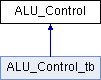
\includegraphics[height=2.000000cm]{class_a_l_u___control}
\end{center}
\end{figure}
\subsection*{Entities}
\begin{DoxyCompactItemize}
\item 
\hyperlink{class_a_l_u___control_1_1_behavioral}{Behavioral} architecture
\begin{DoxyCompactList}\small\item\em This is the \hyperlink{class_a_l_u}{A\-L\-U} control that generates the 4 control bits for the \hyperlink{class_a_l_u}{A\-L\-U}. \end{DoxyCompactList}\end{DoxyCompactItemize}
\subsection*{Ports}
 \begin{DoxyCompactItemize}
\item 
\hyperlink{class_a_l_u___control_ab6a5d61e888c23ba77524db9a1b57d00}{A\-L\-U\-\_\-\-O\-P}  {\bfseries {\bfseries \textcolor{vhdlkeyword}{in}\textcolor{vhdlchar}{ }}} {\bfseries \textcolor{comment}{S\-T\-D\-\_\-logic\-\_\-vector}\textcolor{vhdlchar}{ }\textcolor{vhdlchar}{(}\textcolor{vhdlchar}{ }\textcolor{vhdlchar}{ } \textcolor{vhdldigit}{1} \textcolor{vhdlchar}{ }\textcolor{vhdlchar}{ }\textcolor{vhdlchar}{ }\textcolor{vhdlkeyword}{downto}\textcolor{vhdlchar}{ }\textcolor{vhdlchar}{ }\textcolor{vhdlchar}{ } \textcolor{vhdldigit}{0} \textcolor{vhdlchar}{ }\textcolor{vhdlchar}{)}\textcolor{vhdlchar}{ }} 
\begin{DoxyCompactList}\small\item\em Opcode from controller. \end{DoxyCompactList}\item 
\hyperlink{class_a_l_u___control_a7a955f01ce8523310216d431d36b3355}{A\-L\-U\-\_\-\-Funct\-\_\-\-In}  {\bfseries {\bfseries \textcolor{vhdlkeyword}{in}\textcolor{vhdlchar}{ }}} {\bfseries \textcolor{comment}{S\-T\-D\-\_\-\-L\-O\-G\-I\-C\-\_\-\-V\-E\-C\-T\-O\-R}\textcolor{vhdlchar}{ }\textcolor{vhdlchar}{(}\textcolor{vhdlchar}{ }\textcolor{vhdlchar}{ } \textcolor{vhdldigit}{5} \textcolor{vhdlchar}{ }\textcolor{vhdlchar}{ }\textcolor{vhdlchar}{ }\textcolor{vhdlkeyword}{downto}\textcolor{vhdlchar}{ }\textcolor{vhdlchar}{ }\textcolor{vhdlchar}{ } \textcolor{vhdldigit}{0} \textcolor{vhdlchar}{ }\textcolor{vhdlchar}{)}\textcolor{vhdlchar}{ }} 
\begin{DoxyCompactList}\small\item\em funt\-\_\-in from instruction (first 6 bits) \end{DoxyCompactList}\item 
\hyperlink{class_a_l_u___control_a8ec3ba373cae4fe06c7d82b2ce12561f}{A\-L\-U\-\_\-\-Control\-\_\-out}  {\bfseries {\bfseries \textcolor{vhdlkeyword}{out}\textcolor{vhdlchar}{ }}} {\bfseries \textcolor{comment}{S\-T\-D\-\_\-\-L\-O\-G\-I\-C\-\_\-\-V\-E\-C\-T\-O\-R}\textcolor{vhdlchar}{ }\textcolor{vhdlchar}{(}\textcolor{vhdlchar}{ }\textcolor{vhdlchar}{ } \textcolor{vhdldigit}{3} \textcolor{vhdlchar}{ }\textcolor{vhdlchar}{ }\textcolor{vhdlchar}{ }\textcolor{vhdlkeyword}{downto}\textcolor{vhdlchar}{ }\textcolor{vhdlchar}{ }\textcolor{vhdlchar}{ } \textcolor{vhdldigit}{0} \textcolor{vhdlchar}{ }\textcolor{vhdlchar}{)}\textcolor{vhdlchar}{ }} 
\begin{DoxyCompactList}\small\item\em alu\-\_\-control output \end{DoxyCompactList}\end{DoxyCompactItemize}


\subsection{Detailed Description}
the \hyperlink{class_a_l_u___control}{A\-L\-U\-\_\-\-Control} takes as input the 6 first bit\-S from the instruction and the 2 bits code from the controller. It outputs a 4 bits code to control the \hyperlink{class_a_l_u}{A\-L\-U} 

\subsection{Member Data Documentation}
\hypertarget{class_a_l_u___control_a8ec3ba373cae4fe06c7d82b2ce12561f}{\index{A\-L\-U\-\_\-\-Control@{A\-L\-U\-\_\-\-Control}!A\-L\-U\-\_\-\-Control\-\_\-out@{A\-L\-U\-\_\-\-Control\-\_\-out}}
\index{A\-L\-U\-\_\-\-Control\-\_\-out@{A\-L\-U\-\_\-\-Control\-\_\-out}!ALU_Control@{A\-L\-U\-\_\-\-Control}}
\subsubsection[{A\-L\-U\-\_\-\-Control\-\_\-out}]{\setlength{\rightskip}{0pt plus 5cm}{\bf A\-L\-U\-\_\-\-Control\-\_\-out} {\bfseries \textcolor{vhdlkeyword}{out}\textcolor{vhdlchar}{ }} {\bfseries \textcolor{comment}{S\-T\-D\-\_\-\-L\-O\-G\-I\-C\-\_\-\-V\-E\-C\-T\-O\-R}\textcolor{vhdlchar}{ }\textcolor{vhdlchar}{(}\textcolor{vhdlchar}{ }\textcolor{vhdlchar}{ } \textcolor{vhdldigit}{3} \textcolor{vhdlchar}{ }\textcolor{vhdlchar}{ }\textcolor{vhdlchar}{ }\textcolor{vhdlkeyword}{downto}\textcolor{vhdlchar}{ }\textcolor{vhdlchar}{ }\textcolor{vhdlchar}{ } \textcolor{vhdldigit}{0} \textcolor{vhdlchar}{ }\textcolor{vhdlchar}{)}\textcolor{vhdlchar}{ }} \hspace{0.3cm}{\ttfamily [Port]}}}\label{class_a_l_u___control_a8ec3ba373cae4fe06c7d82b2ce12561f}


alu\-\_\-control output 

\hypertarget{class_a_l_u___control_a7a955f01ce8523310216d431d36b3355}{\index{A\-L\-U\-\_\-\-Control@{A\-L\-U\-\_\-\-Control}!A\-L\-U\-\_\-\-Funct\-\_\-\-In@{A\-L\-U\-\_\-\-Funct\-\_\-\-In}}
\index{A\-L\-U\-\_\-\-Funct\-\_\-\-In@{A\-L\-U\-\_\-\-Funct\-\_\-\-In}!ALU_Control@{A\-L\-U\-\_\-\-Control}}
\subsubsection[{A\-L\-U\-\_\-\-Funct\-\_\-\-In}]{\setlength{\rightskip}{0pt plus 5cm}{\bf A\-L\-U\-\_\-\-Funct\-\_\-\-In} {\bfseries \textcolor{vhdlkeyword}{in}\textcolor{vhdlchar}{ }} {\bfseries \textcolor{comment}{S\-T\-D\-\_\-\-L\-O\-G\-I\-C\-\_\-\-V\-E\-C\-T\-O\-R}\textcolor{vhdlchar}{ }\textcolor{vhdlchar}{(}\textcolor{vhdlchar}{ }\textcolor{vhdlchar}{ } \textcolor{vhdldigit}{5} \textcolor{vhdlchar}{ }\textcolor{vhdlchar}{ }\textcolor{vhdlchar}{ }\textcolor{vhdlkeyword}{downto}\textcolor{vhdlchar}{ }\textcolor{vhdlchar}{ }\textcolor{vhdlchar}{ } \textcolor{vhdldigit}{0} \textcolor{vhdlchar}{ }\textcolor{vhdlchar}{)}\textcolor{vhdlchar}{ }} \hspace{0.3cm}{\ttfamily [Port]}}}\label{class_a_l_u___control_a7a955f01ce8523310216d431d36b3355}


funt\-\_\-in from instruction (first 6 bits) 

\hypertarget{class_a_l_u___control_ab6a5d61e888c23ba77524db9a1b57d00}{\index{A\-L\-U\-\_\-\-Control@{A\-L\-U\-\_\-\-Control}!A\-L\-U\-\_\-\-O\-P@{A\-L\-U\-\_\-\-O\-P}}
\index{A\-L\-U\-\_\-\-O\-P@{A\-L\-U\-\_\-\-O\-P}!ALU_Control@{A\-L\-U\-\_\-\-Control}}
\subsubsection[{A\-L\-U\-\_\-\-O\-P}]{\setlength{\rightskip}{0pt plus 5cm}{\bf A\-L\-U\-\_\-\-O\-P} {\bfseries \textcolor{vhdlkeyword}{in}\textcolor{vhdlchar}{ }} {\bfseries \textcolor{comment}{S\-T\-D\-\_\-logic\-\_\-vector}\textcolor{vhdlchar}{ }\textcolor{vhdlchar}{(}\textcolor{vhdlchar}{ }\textcolor{vhdlchar}{ } \textcolor{vhdldigit}{1} \textcolor{vhdlchar}{ }\textcolor{vhdlchar}{ }\textcolor{vhdlchar}{ }\textcolor{vhdlkeyword}{downto}\textcolor{vhdlchar}{ }\textcolor{vhdlchar}{ }\textcolor{vhdlchar}{ } \textcolor{vhdldigit}{0} \textcolor{vhdlchar}{ }\textcolor{vhdlchar}{)}\textcolor{vhdlchar}{ }} \hspace{0.3cm}{\ttfamily [Port]}}}\label{class_a_l_u___control_ab6a5d61e888c23ba77524db9a1b57d00}


Opcode from controller. 



The documentation for this class was generated from the following file\-:\begin{DoxyCompactItemize}
\item 
documenten/\-Codes/\-M\-I\-P\-S\-\_\-processor/\hyperlink{_a_l_u_control_8vhd}{A\-L\-U\-Control.\-vhd}\end{DoxyCompactItemize}

\hypertarget{class_a_l_u___control__tb}{\section{\-A\-L\-U\-\_\-\-Control\-\_\-tb \-Entity \-Reference}
\label{class_a_l_u___control__tb}\index{\-A\-L\-U\-\_\-\-Control\-\_\-tb@{\-A\-L\-U\-\_\-\-Control\-\_\-tb}}
}
\subsection*{\-Entities}
\begin{DoxyCompactItemize}
\item 
\hyperlink{class_a_l_u___control__tb_1_1behavior}{behavior} architecture
\end{DoxyCompactItemize}


\-The documentation for this class was generated from the following file\-:\begin{DoxyCompactItemize}
\item 
testbenches/\-A\-L\-U\-\_\-\-Control\-\_\-tb.\-vhd\end{DoxyCompactItemize}

\hypertarget{class_a_l_u__tb}{\section{\-A\-L\-U\-\_\-tb \-Entity \-Reference}
\label{class_a_l_u__tb}\index{\-A\-L\-U\-\_\-tb@{\-A\-L\-U\-\_\-tb}}
}
\subsection*{\-Entities}
\begin{DoxyCompactItemize}
\item 
\hyperlink{class_a_l_u__tb_1_1behavior}{behavior} architecture
\end{DoxyCompactItemize}


\-The documentation for this class was generated from the following file\-:\begin{DoxyCompactItemize}
\item 
testbenches/\hyperlink{_a_l_u__tb_8vhd}{\-A\-L\-U\-\_\-tb.\-vhd}\end{DoxyCompactItemize}

\hypertarget{classjump__adder__tb_1_1behavior}{\section{behavior \-Architecture \-Reference}
\label{classjump__adder__tb_1_1behavior}\index{behavior@{behavior}}
}
\*
\*
\subsection*{\-Processes}
 \begin{DoxyCompactItemize}
\item 
\hyperlink{classjump__adder__tb_1_1behavior_ac5bb218131b813f7908ec89476b31fca}{clk\-\_\-process}{\bfseries  (  )}
\item 
\hyperlink{classjump__adder__tb_1_1behavior_ad2efa6785cff833c341e27596b21aeb5}{stim\-\_\-proc}{\bfseries  (  )}
\end{DoxyCompactItemize}
\subsection*{\-Components}
 \begin{DoxyCompactItemize}
\item 
\hyperlink{classjump__adder__tb_1_1behavior_a37126d0718abf44f03b24857c0ce1ea0}{jump\-\_\-adder}  {\bfseries }  
\end{DoxyCompactItemize}
\subsection*{\-Constants}
 \begin{DoxyCompactItemize}
\item 
\hyperlink{classjump__adder__tb_1_1behavior_a3ffd56257467a8089d6f08ff6c8d0755}{clk\-\_\-period} {\bfseries time  \-:=  10  ns } 
\end{DoxyCompactItemize}
\subsection*{\-Signals}
 \begin{DoxyCompactItemize}
\item 
\hyperlink{classjump__adder__tb_1_1behavior_abac182a083cb1fbdec9988ea49b83305}{clk} {\bfseries std\-\_\-logic  \-:= '  0  ' } 
\item 
\hyperlink{classjump__adder__tb_1_1behavior_a6a7e83159e031a9cd68e875f93591ab2}{instruction} {\bfseries std\-\_\-logic\-\_\-vector (   31    downto    0  )  \-:= (  others  = $>$ '  0  '  ) } 
\item 
\hyperlink{classjump__adder__tb_1_1behavior_a00dfa7e780d02a4939d1f6ed4a60541b}{jmp\-\_\-offset} {\bfseries std\-\_\-logic\-\_\-vector (   31    downto    0  )  \-:= (  others  = $>$ '  0  '  ) } 
\item 
\hyperlink{classjump__adder__tb_1_1behavior_afb052939be0f788cfe696c87ec9a06d9}{jmp\-\_\-adress} {\bfseries std\-\_\-logic\-\_\-vector (   31    downto    0  ) } 
\end{DoxyCompactItemize}


\subsection{\-Member \-Function \-Documentation}
\hypertarget{classjump__adder__tb_1_1behavior_ac5bb218131b813f7908ec89476b31fca}{\index{jump\-\_\-adder\-\_\-tb\-::behavior@{jump\-\_\-adder\-\_\-tb\-::behavior}!clk\-\_\-process@{clk\-\_\-process}}
\index{clk\-\_\-process@{clk\-\_\-process}!jump_adder_tb::behavior@{jump\-\_\-adder\-\_\-tb\-::behavior}}
\subsubsection[{clk\-\_\-process}]{\setlength{\rightskip}{0pt plus 5cm}clk\-\_\-process (
\begin{DoxyParamCaption}
{}
\end{DoxyParamCaption}
)\hspace{0.3cm}{\ttfamily  \mbox{[}get\mbox{]}}}}\label{classjump__adder__tb_1_1behavior_ac5bb218131b813f7908ec89476b31fca}
\hypertarget{classjump__adder__tb_1_1behavior_ad2efa6785cff833c341e27596b21aeb5}{\index{jump\-\_\-adder\-\_\-tb\-::behavior@{jump\-\_\-adder\-\_\-tb\-::behavior}!stim\-\_\-proc@{stim\-\_\-proc}}
\index{stim\-\_\-proc@{stim\-\_\-proc}!jump_adder_tb::behavior@{jump\-\_\-adder\-\_\-tb\-::behavior}}
\subsubsection[{stim\-\_\-proc}]{\setlength{\rightskip}{0pt plus 5cm} {\bfseries  } stim\-\_\-proc ( ) \hspace{0.3cm}{\ttfamily  \mbox{[}\-Process\mbox{]}}}}\label{classjump__adder__tb_1_1behavior_ad2efa6785cff833c341e27596b21aeb5}


\subsection{\-Member \-Data \-Documentation}
\hypertarget{classjump__adder__tb_1_1behavior_a37126d0718abf44f03b24857c0ce1ea0}{\index{jump\-\_\-adder\-\_\-tb\-::behavior@{jump\-\_\-adder\-\_\-tb\-::behavior}!jump\-\_\-adder@{jump\-\_\-adder}}
\index{jump\-\_\-adder@{jump\-\_\-adder}!jump_adder_tb::behavior@{jump\-\_\-adder\-\_\-tb\-::behavior}}
\subsubsection[{jump\-\_\-adder}]{\setlength{\rightskip}{0pt plus 5cm}{\bf jump\-\_\-adder} {\bfseries  } \hspace{0.3cm}{\ttfamily  \mbox{[}\-Component\mbox{]}}}}\label{classjump__adder__tb_1_1behavior_a37126d0718abf44f03b24857c0ce1ea0}
\hypertarget{classjump__adder__tb_1_1behavior_abac182a083cb1fbdec9988ea49b83305}{\index{jump\-\_\-adder\-\_\-tb\-::behavior@{jump\-\_\-adder\-\_\-tb\-::behavior}!clk@{clk}}
\index{clk@{clk}!jump_adder_tb::behavior@{jump\-\_\-adder\-\_\-tb\-::behavior}}
\subsubsection[{clk}]{\setlength{\rightskip}{0pt plus 5cm}{\bf clk} {\bfseries std\-\_\-logic  \-:= '  0  ' } \hspace{0.3cm}{\ttfamily  \mbox{[}\-Signal\mbox{]}}}}\label{classjump__adder__tb_1_1behavior_abac182a083cb1fbdec9988ea49b83305}
\hypertarget{classjump__adder__tb_1_1behavior_a6a7e83159e031a9cd68e875f93591ab2}{\index{jump\-\_\-adder\-\_\-tb\-::behavior@{jump\-\_\-adder\-\_\-tb\-::behavior}!instruction@{instruction}}
\index{instruction@{instruction}!jump_adder_tb::behavior@{jump\-\_\-adder\-\_\-tb\-::behavior}}
\subsubsection[{instruction}]{\setlength{\rightskip}{0pt plus 5cm}{\bf instruction} {\bfseries std\-\_\-logic\-\_\-vector (   31    downto    0  )  \-:= (  others  = $>$ '  0  '  ) } \hspace{0.3cm}{\ttfamily  \mbox{[}\-Signal\mbox{]}}}}\label{classjump__adder__tb_1_1behavior_a6a7e83159e031a9cd68e875f93591ab2}
\hypertarget{classjump__adder__tb_1_1behavior_a00dfa7e780d02a4939d1f6ed4a60541b}{\index{jump\-\_\-adder\-\_\-tb\-::behavior@{jump\-\_\-adder\-\_\-tb\-::behavior}!jmp\-\_\-offset@{jmp\-\_\-offset}}
\index{jmp\-\_\-offset@{jmp\-\_\-offset}!jump_adder_tb::behavior@{jump\-\_\-adder\-\_\-tb\-::behavior}}
\subsubsection[{jmp\-\_\-offset}]{\setlength{\rightskip}{0pt plus 5cm}{\bf jmp\-\_\-offset} {\bfseries std\-\_\-logic\-\_\-vector (   31    downto    0  )  \-:= (  others  = $>$ '  0  '  ) } \hspace{0.3cm}{\ttfamily  \mbox{[}\-Signal\mbox{]}}}}\label{classjump__adder__tb_1_1behavior_a00dfa7e780d02a4939d1f6ed4a60541b}
\hypertarget{classjump__adder__tb_1_1behavior_afb052939be0f788cfe696c87ec9a06d9}{\index{jump\-\_\-adder\-\_\-tb\-::behavior@{jump\-\_\-adder\-\_\-tb\-::behavior}!jmp\-\_\-adress@{jmp\-\_\-adress}}
\index{jmp\-\_\-adress@{jmp\-\_\-adress}!jump_adder_tb::behavior@{jump\-\_\-adder\-\_\-tb\-::behavior}}
\subsubsection[{jmp\-\_\-adress}]{\setlength{\rightskip}{0pt plus 5cm}{\bf jmp\-\_\-adress} {\bfseries std\-\_\-logic\-\_\-vector (   31    downto    0  ) } \hspace{0.3cm}{\ttfamily  \mbox{[}\-Signal\mbox{]}}}}\label{classjump__adder__tb_1_1behavior_afb052939be0f788cfe696c87ec9a06d9}
\hypertarget{classjump__adder__tb_1_1behavior_a3ffd56257467a8089d6f08ff6c8d0755}{\index{jump\-\_\-adder\-\_\-tb\-::behavior@{jump\-\_\-adder\-\_\-tb\-::behavior}!clk\-\_\-period@{clk\-\_\-period}}
\index{clk\-\_\-period@{clk\-\_\-period}!jump_adder_tb::behavior@{jump\-\_\-adder\-\_\-tb\-::behavior}}
\subsubsection[{clk\-\_\-period}]{\setlength{\rightskip}{0pt plus 5cm}{\bf clk\-\_\-period} {\bfseries time  \-:=  10  ns } \hspace{0.3cm}{\ttfamily  \mbox{[}\-Constant\mbox{]}}}}\label{classjump__adder__tb_1_1behavior_a3ffd56257467a8089d6f08ff6c8d0755}


\-The documentation for this class was generated from the following files\-:\begin{DoxyCompactItemize}
\item 
testbenches/\hyperlink{jump__adder__tb_8vhd}{jump\-\_\-adder\-\_\-tb.\-vhd}\end{DoxyCompactItemize}

\hypertarget{classmips__proc__tb_1_1behavior}{\section{behavior \-Architecture \-Reference}
\label{classmips__proc__tb_1_1behavior}\index{behavior@{behavior}}
}
\*
\*
\subsection*{\-Processes}
 \begin{DoxyCompactItemize}
\item 
\hypertarget{classmips__proc__tb_1_1behavior_ac5bb218131b813f7908ec89476b31fca}{\hyperlink{classmips__proc__tb_1_1behavior_ac5bb218131b813f7908ec89476b31fca}{clk\-\_\-process}{\bfseries  (  )}}\label{classmips__proc__tb_1_1behavior_ac5bb218131b813f7908ec89476b31fca}

\item 
\hypertarget{classmips__proc__tb_1_1behavior_ad2efa6785cff833c341e27596b21aeb5}{\hyperlink{classmips__proc__tb_1_1behavior_ad2efa6785cff833c341e27596b21aeb5}{stim\-\_\-proc}{\bfseries  (  )}}\label{classmips__proc__tb_1_1behavior_ad2efa6785cff833c341e27596b21aeb5}

\end{DoxyCompactItemize}
\subsection*{\-Components}
 \begin{DoxyCompactItemize}
\item 
\hypertarget{classmips__proc__tb_1_1behavior_aade1eeda70a966f797de9864493345a7}{\hyperlink{classmips__proc__tb_1_1behavior_aade1eeda70a966f797de9864493345a7}{mips\-\_\-proc}  {\bfseries }  }\label{classmips__proc__tb_1_1behavior_aade1eeda70a966f797de9864493345a7}

\end{DoxyCompactItemize}
\subsection*{\-Constants}
 \begin{DoxyCompactItemize}
\item 
\hypertarget{classmips__proc__tb_1_1behavior_a5f1272460f402ee58f04009a62af525e}{\hyperlink{classmips__proc__tb_1_1behavior_a5f1272460f402ee58f04009a62af525e}{clk\-\_\-period} {\bfseries time  \-:=  10  ns } }\label{classmips__proc__tb_1_1behavior_a5f1272460f402ee58f04009a62af525e}

\end{DoxyCompactItemize}
\subsection*{\-Signals}
 \begin{DoxyCompactItemize}
\item 
\hypertarget{classmips__proc__tb_1_1behavior_a6732b1e05ec0cbac56a07dc48f391fd8}{\hyperlink{classmips__proc__tb_1_1behavior_a6732b1e05ec0cbac56a07dc48f391fd8}{clk} {\bfseries std\-\_\-logic  \-:= '  0  ' } }\label{classmips__proc__tb_1_1behavior_a6732b1e05ec0cbac56a07dc48f391fd8}

\item 
\hypertarget{classmips__proc__tb_1_1behavior_a1227312426e741edc82659864d673dd7}{\hyperlink{classmips__proc__tb_1_1behavior_a1227312426e741edc82659864d673dd7}{reset} {\bfseries std\-\_\-logic  \-:= '  0  ' } }\label{classmips__proc__tb_1_1behavior_a1227312426e741edc82659864d673dd7}

\item 
\hypertarget{classmips__proc__tb_1_1behavior_a46c7e46ecf9add8594bee7c639ee1fe1}{\hyperlink{classmips__proc__tb_1_1behavior_a46c7e46ecf9add8594bee7c639ee1fe1}{instruction} {\bfseries std\-\_\-logic\-\_\-vector (   31    downto    0  ) } }\label{classmips__proc__tb_1_1behavior_a46c7e46ecf9add8594bee7c639ee1fe1}

\item 
\hypertarget{classmips__proc__tb_1_1behavior_a9ab65ec266e93aca6fc7f8ce688f92bf}{\hyperlink{classmips__proc__tb_1_1behavior_a9ab65ec266e93aca6fc7f8ce688f92bf}{pca\-\_\-o} {\bfseries std\-\_\-logic\-\_\-vector (   31    downto    0  ) } }\label{classmips__proc__tb_1_1behavior_a9ab65ec266e93aca6fc7f8ce688f92bf}

\end{DoxyCompactItemize}


\-The documentation for this class was generated from the following files\-:\begin{DoxyCompactItemize}
\item 
testbenches/mips\-\_\-proc\-\_\-tb.\-vhd\end{DoxyCompactItemize}

\hypertarget{classmux__tb_1_1behavior}{\section{behavior \-Architecture \-Reference}
\label{classmux__tb_1_1behavior}\index{behavior@{behavior}}
}
\*
\*
\subsection*{\-Processes}
 \begin{DoxyCompactItemize}
\item 
\hyperlink{classmux__tb_1_1behavior_ac5bb218131b813f7908ec89476b31fca}{clk\-\_\-process}{\bfseries  (  )}
\item 
\hyperlink{classmux__tb_1_1behavior_ad2efa6785cff833c341e27596b21aeb5}{stim\-\_\-proc}{\bfseries  (  )}
\end{DoxyCompactItemize}
\subsection*{\-Components}
 \begin{DoxyCompactItemize}
\item 
\hyperlink{classmux__tb_1_1behavior_a73760dea8da2e6f41a8c18e8bf78aa35}{\-M\-U\-X}  {\bfseries }  
\end{DoxyCompactItemize}
\subsection*{\-Constants}
 \begin{DoxyCompactItemize}
\item 
\hyperlink{classmux__tb_1_1behavior_a204a2fe2cd2e77cb28f30aeab011e19e}{clk\-\_\-period} {\bfseries time  \-:=  10  ns } 
\end{DoxyCompactItemize}
\subsection*{\-Signals}
 \begin{DoxyCompactItemize}
\item 
\hyperlink{classmux__tb_1_1behavior_aa4a50c298077fcba21ee7b8037fae196}{clk} {\bfseries std\-\_\-logic  \-:= '  0  ' } 
\item 
\hyperlink{classmux__tb_1_1behavior_aafcce8e7a57f78ec316c2d09baaf938d}{tb\-\_\-vec\-\_\-in\-\_\-1} {\bfseries std\-\_\-logic\-\_\-vector (   31    downto    0  ) } 
\item 
\hyperlink{classmux__tb_1_1behavior_ab2752542a9d10d877b272c9484b29df9}{tb\-\_\-vec\-\_\-in\-\_\-2} {\bfseries std\-\_\-logic\-\_\-vector (   31    downto    0  ) } 
\item 
\hyperlink{classmux__tb_1_1behavior_a25ec99ba02878236496471f1c0b4aca1}{tb\-\_\-selector} {\bfseries std\-\_\-logic } 
\item 
\hyperlink{classmux__tb_1_1behavior_a1ef2cbfab26351585dd50c0f22be5fa6}{tb\-\_\-vec\-\_\-out} {\bfseries std\-\_\-logic\-\_\-vector (   31    downto    0  ) } 
\end{DoxyCompactItemize}


\subsection{\-Member \-Function \-Documentation}
\hypertarget{classmux__tb_1_1behavior_ac5bb218131b813f7908ec89476b31fca}{\index{mux\-\_\-tb\-::behavior@{mux\-\_\-tb\-::behavior}!clk\-\_\-process@{clk\-\_\-process}}
\index{clk\-\_\-process@{clk\-\_\-process}!mux_tb::behavior@{mux\-\_\-tb\-::behavior}}
\subsubsection[{clk\-\_\-process}]{\setlength{\rightskip}{0pt plus 5cm}clk\-\_\-process (
\begin{DoxyParamCaption}
{}
\end{DoxyParamCaption}
)\hspace{0.3cm}{\ttfamily  \mbox{[}get\mbox{]}}}}\label{classmux__tb_1_1behavior_ac5bb218131b813f7908ec89476b31fca}
\hypertarget{classmux__tb_1_1behavior_ad2efa6785cff833c341e27596b21aeb5}{\index{mux\-\_\-tb\-::behavior@{mux\-\_\-tb\-::behavior}!stim\-\_\-proc@{stim\-\_\-proc}}
\index{stim\-\_\-proc@{stim\-\_\-proc}!mux_tb::behavior@{mux\-\_\-tb\-::behavior}}
\subsubsection[{stim\-\_\-proc}]{\setlength{\rightskip}{0pt plus 5cm} {\bfseries  } stim\-\_\-proc ( ) \hspace{0.3cm}{\ttfamily  \mbox{[}\-Process\mbox{]}}}}\label{classmux__tb_1_1behavior_ad2efa6785cff833c341e27596b21aeb5}


\subsection{\-Member \-Data \-Documentation}
\hypertarget{classmux__tb_1_1behavior_a73760dea8da2e6f41a8c18e8bf78aa35}{\index{mux\-\_\-tb\-::behavior@{mux\-\_\-tb\-::behavior}!\-M\-U\-X@{\-M\-U\-X}}
\index{\-M\-U\-X@{\-M\-U\-X}!mux_tb::behavior@{mux\-\_\-tb\-::behavior}}
\subsubsection[{\-M\-U\-X}]{\setlength{\rightskip}{0pt plus 5cm}{\bf \-M\-U\-X} {\bfseries  } \hspace{0.3cm}{\ttfamily  \mbox{[}\-Component\mbox{]}}}}\label{classmux__tb_1_1behavior_a73760dea8da2e6f41a8c18e8bf78aa35}
\hypertarget{classmux__tb_1_1behavior_aa4a50c298077fcba21ee7b8037fae196}{\index{mux\-\_\-tb\-::behavior@{mux\-\_\-tb\-::behavior}!clk@{clk}}
\index{clk@{clk}!mux_tb::behavior@{mux\-\_\-tb\-::behavior}}
\subsubsection[{clk}]{\setlength{\rightskip}{0pt plus 5cm}{\bf clk} {\bfseries std\-\_\-logic  \-:= '  0  ' } \hspace{0.3cm}{\ttfamily  \mbox{[}\-Signal\mbox{]}}}}\label{classmux__tb_1_1behavior_aa4a50c298077fcba21ee7b8037fae196}
\hypertarget{classmux__tb_1_1behavior_aafcce8e7a57f78ec316c2d09baaf938d}{\index{mux\-\_\-tb\-::behavior@{mux\-\_\-tb\-::behavior}!tb\-\_\-vec\-\_\-in\-\_\-1@{tb\-\_\-vec\-\_\-in\-\_\-1}}
\index{tb\-\_\-vec\-\_\-in\-\_\-1@{tb\-\_\-vec\-\_\-in\-\_\-1}!mux_tb::behavior@{mux\-\_\-tb\-::behavior}}
\subsubsection[{tb\-\_\-vec\-\_\-in\-\_\-1}]{\setlength{\rightskip}{0pt plus 5cm}{\bf tb\-\_\-vec\-\_\-in\-\_\-1} {\bfseries std\-\_\-logic\-\_\-vector (   31    downto    0  ) } \hspace{0.3cm}{\ttfamily  \mbox{[}\-Signal\mbox{]}}}}\label{classmux__tb_1_1behavior_aafcce8e7a57f78ec316c2d09baaf938d}
\hypertarget{classmux__tb_1_1behavior_ab2752542a9d10d877b272c9484b29df9}{\index{mux\-\_\-tb\-::behavior@{mux\-\_\-tb\-::behavior}!tb\-\_\-vec\-\_\-in\-\_\-2@{tb\-\_\-vec\-\_\-in\-\_\-2}}
\index{tb\-\_\-vec\-\_\-in\-\_\-2@{tb\-\_\-vec\-\_\-in\-\_\-2}!mux_tb::behavior@{mux\-\_\-tb\-::behavior}}
\subsubsection[{tb\-\_\-vec\-\_\-in\-\_\-2}]{\setlength{\rightskip}{0pt plus 5cm}{\bf tb\-\_\-vec\-\_\-in\-\_\-2} {\bfseries std\-\_\-logic\-\_\-vector (   31    downto    0  ) } \hspace{0.3cm}{\ttfamily  \mbox{[}\-Signal\mbox{]}}}}\label{classmux__tb_1_1behavior_ab2752542a9d10d877b272c9484b29df9}
\hypertarget{classmux__tb_1_1behavior_a25ec99ba02878236496471f1c0b4aca1}{\index{mux\-\_\-tb\-::behavior@{mux\-\_\-tb\-::behavior}!tb\-\_\-selector@{tb\-\_\-selector}}
\index{tb\-\_\-selector@{tb\-\_\-selector}!mux_tb::behavior@{mux\-\_\-tb\-::behavior}}
\subsubsection[{tb\-\_\-selector}]{\setlength{\rightskip}{0pt plus 5cm}{\bf tb\-\_\-selector} {\bfseries std\-\_\-logic } \hspace{0.3cm}{\ttfamily  \mbox{[}\-Signal\mbox{]}}}}\label{classmux__tb_1_1behavior_a25ec99ba02878236496471f1c0b4aca1}
\hypertarget{classmux__tb_1_1behavior_a1ef2cbfab26351585dd50c0f22be5fa6}{\index{mux\-\_\-tb\-::behavior@{mux\-\_\-tb\-::behavior}!tb\-\_\-vec\-\_\-out@{tb\-\_\-vec\-\_\-out}}
\index{tb\-\_\-vec\-\_\-out@{tb\-\_\-vec\-\_\-out}!mux_tb::behavior@{mux\-\_\-tb\-::behavior}}
\subsubsection[{tb\-\_\-vec\-\_\-out}]{\setlength{\rightskip}{0pt plus 5cm}{\bf tb\-\_\-vec\-\_\-out} {\bfseries std\-\_\-logic\-\_\-vector (   31    downto    0  ) } \hspace{0.3cm}{\ttfamily  \mbox{[}\-Signal\mbox{]}}}}\label{classmux__tb_1_1behavior_a1ef2cbfab26351585dd50c0f22be5fa6}
\hypertarget{classmux__tb_1_1behavior_a204a2fe2cd2e77cb28f30aeab011e19e}{\index{mux\-\_\-tb\-::behavior@{mux\-\_\-tb\-::behavior}!clk\-\_\-period@{clk\-\_\-period}}
\index{clk\-\_\-period@{clk\-\_\-period}!mux_tb::behavior@{mux\-\_\-tb\-::behavior}}
\subsubsection[{clk\-\_\-period}]{\setlength{\rightskip}{0pt plus 5cm}{\bf clk\-\_\-period} {\bfseries time  \-:=  10  ns } \hspace{0.3cm}{\ttfamily  \mbox{[}\-Constant\mbox{]}}}}\label{classmux__tb_1_1behavior_a204a2fe2cd2e77cb28f30aeab011e19e}


\-The documentation for this class was generated from the following files\-:\begin{DoxyCompactItemize}
\item 
testbenches/\hyperlink{mux__tb_8vhd}{mux\-\_\-tb.\-vhd}\end{DoxyCompactItemize}

\hypertarget{class_p_c_adder__tb_1_1behavior}{\section{behavior \-Architecture \-Reference}
\label{class_p_c_adder__tb_1_1behavior}\index{behavior@{behavior}}
}
\*
\*
\subsection*{\-Processes}
 \begin{DoxyCompactItemize}
\item 
\hypertarget{class_p_c_adder__tb_1_1behavior_ac5bb218131b813f7908ec89476b31fca}{\hyperlink{class_p_c_adder__tb_1_1behavior_ac5bb218131b813f7908ec89476b31fca}{clk\-\_\-process}{\bfseries  (  )}}\label{class_p_c_adder__tb_1_1behavior_ac5bb218131b813f7908ec89476b31fca}

\item 
\hypertarget{class_p_c_adder__tb_1_1behavior_ad2efa6785cff833c341e27596b21aeb5}{\hyperlink{class_p_c_adder__tb_1_1behavior_ad2efa6785cff833c341e27596b21aeb5}{stim\-\_\-proc}{\bfseries  (  )}}\label{class_p_c_adder__tb_1_1behavior_ad2efa6785cff833c341e27596b21aeb5}

\end{DoxyCompactItemize}
\subsection*{\-Components}
 \begin{DoxyCompactItemize}
\item 
\hypertarget{class_p_c_adder__tb_1_1behavior_a5dc0e950c743b6867902097030b977b0}{\hyperlink{class_p_c_adder__tb_1_1behavior_a5dc0e950c743b6867902097030b977b0}{\-P\-C\-A}  {\bfseries }  }\label{class_p_c_adder__tb_1_1behavior_a5dc0e950c743b6867902097030b977b0}

\end{DoxyCompactItemize}
\subsection*{\-Constants}
 \begin{DoxyCompactItemize}
\item 
\hypertarget{class_p_c_adder__tb_1_1behavior_ab3c46918aa1e58060e340ba6e16733a9}{\hyperlink{class_p_c_adder__tb_1_1behavior_ab3c46918aa1e58060e340ba6e16733a9}{clk\-\_\-period} {\bfseries time  \-:=  10  ns } }\label{class_p_c_adder__tb_1_1behavior_ab3c46918aa1e58060e340ba6e16733a9}

\end{DoxyCompactItemize}
\subsection*{\-Signals}
 \begin{DoxyCompactItemize}
\item 
\hypertarget{class_p_c_adder__tb_1_1behavior_ad58a2240944eedcee02839cbcf3f871b}{\hyperlink{class_p_c_adder__tb_1_1behavior_ad58a2240944eedcee02839cbcf3f871b}{clk} {\bfseries std\-\_\-logic } }\label{class_p_c_adder__tb_1_1behavior_ad58a2240944eedcee02839cbcf3f871b}

\item 
\hypertarget{class_p_c_adder__tb_1_1behavior_a41945ec3325c2b38b7618dd164dbc2ef}{\hyperlink{class_p_c_adder__tb_1_1behavior_a41945ec3325c2b38b7618dd164dbc2ef}{\-P\-C} {\bfseries std\-\_\-logic\-\_\-vector (   31    downto    0  )  \-:= (  others  = $>$ '  0  '  ) } }\label{class_p_c_adder__tb_1_1behavior_a41945ec3325c2b38b7618dd164dbc2ef}

\item 
\hypertarget{class_p_c_adder__tb_1_1behavior_a6e9bc854a8af2389b8d808375c044d2f}{\hyperlink{class_p_c_adder__tb_1_1behavior_a6e9bc854a8af2389b8d808375c044d2f}{\-P\-C4} {\bfseries std\-\_\-logic\-\_\-vector (   31    downto    0  ) } }\label{class_p_c_adder__tb_1_1behavior_a6e9bc854a8af2389b8d808375c044d2f}

\end{DoxyCompactItemize}


\-The documentation for this class was generated from the following files\-:\begin{DoxyCompactItemize}
\item 
testbenches/\-P\-C\-Adder\-\_\-tb.\-vhd\end{DoxyCompactItemize}

\hypertarget{class_a_l_u___control__tb_1_1behavior}{\section{behavior \-Architecture \-Reference}
\label{class_a_l_u___control__tb_1_1behavior}\index{behavior@{behavior}}
}
\*
\*
\subsection*{\-Processes}
 \begin{DoxyCompactItemize}
\item 
\hypertarget{class_a_l_u___control__tb_1_1behavior_ac5bb218131b813f7908ec89476b31fca}{\hyperlink{class_a_l_u___control__tb_1_1behavior_ac5bb218131b813f7908ec89476b31fca}{clk\-\_\-process}{\bfseries  (  )}}\label{class_a_l_u___control__tb_1_1behavior_ac5bb218131b813f7908ec89476b31fca}

\item 
\hypertarget{class_a_l_u___control__tb_1_1behavior_ad2efa6785cff833c341e27596b21aeb5}{\hyperlink{class_a_l_u___control__tb_1_1behavior_ad2efa6785cff833c341e27596b21aeb5}{stim\-\_\-proc}{\bfseries  (  )}}\label{class_a_l_u___control__tb_1_1behavior_ad2efa6785cff833c341e27596b21aeb5}

\end{DoxyCompactItemize}
\subsection*{\-Components}
 \begin{DoxyCompactItemize}
\item 
\hypertarget{class_a_l_u___control__tb_1_1behavior_abf60193336988d744deadd38bbf9d27a}{\hyperlink{class_a_l_u___control__tb_1_1behavior_abf60193336988d744deadd38bbf9d27a}{\-A\-L\-U\-\_\-\-Control}  {\bfseries }  }\label{class_a_l_u___control__tb_1_1behavior_abf60193336988d744deadd38bbf9d27a}

\end{DoxyCompactItemize}
\subsection*{\-Constants}
 \begin{DoxyCompactItemize}
\item 
\hypertarget{class_a_l_u___control__tb_1_1behavior_a8a175a7f832828463d31be056e0be9a5}{\hyperlink{class_a_l_u___control__tb_1_1behavior_a8a175a7f832828463d31be056e0be9a5}{clk\-\_\-period} {\bfseries time  \-:=  10  ns } }\label{class_a_l_u___control__tb_1_1behavior_a8a175a7f832828463d31be056e0be9a5}

\end{DoxyCompactItemize}
\subsection*{\-Signals}
 \begin{DoxyCompactItemize}
\item 
\hypertarget{class_a_l_u___control__tb_1_1behavior_a815bf9e542a3c49c6651f755d08a4ac9}{\hyperlink{class_a_l_u___control__tb_1_1behavior_a815bf9e542a3c49c6651f755d08a4ac9}{\-A\-L\-U\-\_\-\-O\-P} {\bfseries std\-\_\-logic\-\_\-vector (   1    downto    0  )  \-:= (  others  = $>$ '  0  '  ) } }\label{class_a_l_u___control__tb_1_1behavior_a815bf9e542a3c49c6651f755d08a4ac9}

\item 
\hypertarget{class_a_l_u___control__tb_1_1behavior_afe12d1d11e7ef94c862d25007711d671}{\hyperlink{class_a_l_u___control__tb_1_1behavior_afe12d1d11e7ef94c862d25007711d671}{\-A\-L\-U\-\_\-\-Funct\-\_\-\-In} {\bfseries std\-\_\-logic\-\_\-vector (   5    downto    0  )  \-:= (  others  = $>$ '  0  '  ) } }\label{class_a_l_u___control__tb_1_1behavior_afe12d1d11e7ef94c862d25007711d671}

\item 
\hypertarget{class_a_l_u___control__tb_1_1behavior_a1b3e29926e973200886940842ebe8876}{\hyperlink{class_a_l_u___control__tb_1_1behavior_a1b3e29926e973200886940842ebe8876}{\-A\-L\-U\-\_\-\-Control\-\_\-out} {\bfseries std\-\_\-logic\-\_\-vector (   3    downto    0  ) } }\label{class_a_l_u___control__tb_1_1behavior_a1b3e29926e973200886940842ebe8876}

\item 
\hypertarget{class_a_l_u___control__tb_1_1behavior_a94eb3ba5e2f4df12778cb4b26b5f9f2e}{\hyperlink{class_a_l_u___control__tb_1_1behavior_a94eb3ba5e2f4df12778cb4b26b5f9f2e}{clk} {\bfseries std\-\_\-logic } }\label{class_a_l_u___control__tb_1_1behavior_a94eb3ba5e2f4df12778cb4b26b5f9f2e}

\end{DoxyCompactItemize}


\-The documentation for this class was generated from the following files\-:\begin{DoxyCompactItemize}
\item 
testbenches/\-A\-L\-U\-\_\-\-Control\-\_\-tb.\-vhd\end{DoxyCompactItemize}

\hypertarget{class_p_counte__tb_1_1behavior}{\section{behavior \-Architecture \-Reference}
\label{class_p_counte__tb_1_1behavior}\index{behavior@{behavior}}
}
\*
\*
\subsection*{\-Processes}
 \begin{DoxyCompactItemize}
\item 
\hyperlink{class_p_counte__tb_1_1behavior_ac5bb218131b813f7908ec89476b31fca}{clk\-\_\-process}{\bfseries  (  )}
\item 
\hyperlink{class_p_counte__tb_1_1behavior_ad2efa6785cff833c341e27596b21aeb5}{stim\-\_\-proc}{\bfseries  (  )}
\end{DoxyCompactItemize}
\subsection*{\-Components}
 \begin{DoxyCompactItemize}
\item 
\hyperlink{class_p_counte__tb_1_1behavior_aaf5ddd6f1a6925eba963bfefa161e9df}{pc}  {\bfseries }  
\end{DoxyCompactItemize}
\subsection*{\-Constants}
 \begin{DoxyCompactItemize}
\item 
\hyperlink{class_p_counte__tb_1_1behavior_a84fbaa8d4f8539ee8577e4f05d006dfb}{clk\-\_\-period} {\bfseries time  \-:=  10  ns } 
\end{DoxyCompactItemize}
\subsection*{\-Signals}
 \begin{DoxyCompactItemize}
\item 
\hyperlink{class_p_counte__tb_1_1behavior_acb38257efabc3b2fa08d2a365cd7ff01}{clk} {\bfseries std\-\_\-logic  \-:= '  0  ' } 
\item 
\hyperlink{class_p_counte__tb_1_1behavior_afedcb12b726c79840717ef89dbe704ed}{reset} {\bfseries std\-\_\-logic  \-:= '  0  ' } 
\item 
\hyperlink{class_p_counte__tb_1_1behavior_ac2dd31bad98644f37a6e62a770f5a5f7}{\-P\-C\-\_\-in} {\bfseries std\-\_\-logic\-\_\-vector (   31    downto    0  )  \-:= (  others  = $>$ '  0  '  ) } 
\item 
\hyperlink{class_p_counte__tb_1_1behavior_a43d3d66618c7e36ea6b882156984c629}{\-P\-C\-\_\-out} {\bfseries std\-\_\-logic\-\_\-vector (   31    downto    0  ) } 
\end{DoxyCompactItemize}


\subsection{\-Member \-Function \-Documentation}
\hypertarget{class_p_counte__tb_1_1behavior_ac5bb218131b813f7908ec89476b31fca}{\index{\-P\-Counte\-\_\-tb\-::behavior@{\-P\-Counte\-\_\-tb\-::behavior}!clk\-\_\-process@{clk\-\_\-process}}
\index{clk\-\_\-process@{clk\-\_\-process}!PCounte_tb::behavior@{\-P\-Counte\-\_\-tb\-::behavior}}
\subsubsection[{clk\-\_\-process}]{\setlength{\rightskip}{0pt plus 5cm}clk\-\_\-process (
\begin{DoxyParamCaption}
{}
\end{DoxyParamCaption}
)\hspace{0.3cm}{\ttfamily  \mbox{[}get\mbox{]}}}}\label{class_p_counte__tb_1_1behavior_ac5bb218131b813f7908ec89476b31fca}
\hypertarget{class_p_counte__tb_1_1behavior_ad2efa6785cff833c341e27596b21aeb5}{\index{\-P\-Counte\-\_\-tb\-::behavior@{\-P\-Counte\-\_\-tb\-::behavior}!stim\-\_\-proc@{stim\-\_\-proc}}
\index{stim\-\_\-proc@{stim\-\_\-proc}!PCounte_tb::behavior@{\-P\-Counte\-\_\-tb\-::behavior}}
\subsubsection[{stim\-\_\-proc}]{\setlength{\rightskip}{0pt plus 5cm} {\bfseries  } stim\-\_\-proc ( ) \hspace{0.3cm}{\ttfamily  \mbox{[}\-Process\mbox{]}}}}\label{class_p_counte__tb_1_1behavior_ad2efa6785cff833c341e27596b21aeb5}


\subsection{\-Member \-Data \-Documentation}
\hypertarget{class_p_counte__tb_1_1behavior_aaf5ddd6f1a6925eba963bfefa161e9df}{\index{\-P\-Counte\-\_\-tb\-::behavior@{\-P\-Counte\-\_\-tb\-::behavior}!pc@{pc}}
\index{pc@{pc}!PCounte_tb::behavior@{\-P\-Counte\-\_\-tb\-::behavior}}
\subsubsection[{pc}]{\setlength{\rightskip}{0pt plus 5cm}{\bf pc} {\bfseries  } \hspace{0.3cm}{\ttfamily  \mbox{[}\-Component\mbox{]}}}}\label{class_p_counte__tb_1_1behavior_aaf5ddd6f1a6925eba963bfefa161e9df}
\hypertarget{class_p_counte__tb_1_1behavior_acb38257efabc3b2fa08d2a365cd7ff01}{\index{\-P\-Counte\-\_\-tb\-::behavior@{\-P\-Counte\-\_\-tb\-::behavior}!clk@{clk}}
\index{clk@{clk}!PCounte_tb::behavior@{\-P\-Counte\-\_\-tb\-::behavior}}
\subsubsection[{clk}]{\setlength{\rightskip}{0pt plus 5cm}{\bf clk} {\bfseries std\-\_\-logic  \-:= '  0  ' } \hspace{0.3cm}{\ttfamily  \mbox{[}\-Signal\mbox{]}}}}\label{class_p_counte__tb_1_1behavior_acb38257efabc3b2fa08d2a365cd7ff01}
\hypertarget{class_p_counte__tb_1_1behavior_afedcb12b726c79840717ef89dbe704ed}{\index{\-P\-Counte\-\_\-tb\-::behavior@{\-P\-Counte\-\_\-tb\-::behavior}!reset@{reset}}
\index{reset@{reset}!PCounte_tb::behavior@{\-P\-Counte\-\_\-tb\-::behavior}}
\subsubsection[{reset}]{\setlength{\rightskip}{0pt plus 5cm}{\bf reset} {\bfseries std\-\_\-logic  \-:= '  0  ' } \hspace{0.3cm}{\ttfamily  \mbox{[}\-Signal\mbox{]}}}}\label{class_p_counte__tb_1_1behavior_afedcb12b726c79840717ef89dbe704ed}
\hypertarget{class_p_counte__tb_1_1behavior_ac2dd31bad98644f37a6e62a770f5a5f7}{\index{\-P\-Counte\-\_\-tb\-::behavior@{\-P\-Counte\-\_\-tb\-::behavior}!\-P\-C\-\_\-in@{\-P\-C\-\_\-in}}
\index{\-P\-C\-\_\-in@{\-P\-C\-\_\-in}!PCounte_tb::behavior@{\-P\-Counte\-\_\-tb\-::behavior}}
\subsubsection[{\-P\-C\-\_\-in}]{\setlength{\rightskip}{0pt plus 5cm}{\bf \-P\-C\-\_\-in} {\bfseries std\-\_\-logic\-\_\-vector (   31    downto    0  )  \-:= (  others  = $>$ '  0  '  ) } \hspace{0.3cm}{\ttfamily  \mbox{[}\-Signal\mbox{]}}}}\label{class_p_counte__tb_1_1behavior_ac2dd31bad98644f37a6e62a770f5a5f7}
\hypertarget{class_p_counte__tb_1_1behavior_a43d3d66618c7e36ea6b882156984c629}{\index{\-P\-Counte\-\_\-tb\-::behavior@{\-P\-Counte\-\_\-tb\-::behavior}!\-P\-C\-\_\-out@{\-P\-C\-\_\-out}}
\index{\-P\-C\-\_\-out@{\-P\-C\-\_\-out}!PCounte_tb::behavior@{\-P\-Counte\-\_\-tb\-::behavior}}
\subsubsection[{\-P\-C\-\_\-out}]{\setlength{\rightskip}{0pt plus 5cm}{\bf \-P\-C\-\_\-out} {\bfseries std\-\_\-logic\-\_\-vector (   31    downto    0  ) } \hspace{0.3cm}{\ttfamily  \mbox{[}\-Signal\mbox{]}}}}\label{class_p_counte__tb_1_1behavior_a43d3d66618c7e36ea6b882156984c629}
\hypertarget{class_p_counte__tb_1_1behavior_a84fbaa8d4f8539ee8577e4f05d006dfb}{\index{\-P\-Counte\-\_\-tb\-::behavior@{\-P\-Counte\-\_\-tb\-::behavior}!clk\-\_\-period@{clk\-\_\-period}}
\index{clk\-\_\-period@{clk\-\_\-period}!PCounte_tb::behavior@{\-P\-Counte\-\_\-tb\-::behavior}}
\subsubsection[{clk\-\_\-period}]{\setlength{\rightskip}{0pt plus 5cm}{\bf clk\-\_\-period} {\bfseries time  \-:=  10  ns } \hspace{0.3cm}{\ttfamily  \mbox{[}\-Constant\mbox{]}}}}\label{class_p_counte__tb_1_1behavior_a84fbaa8d4f8539ee8577e4f05d006dfb}


\-The documentation for this class was generated from the following files\-:\begin{DoxyCompactItemize}
\item 
testbenches/\hyperlink{_p_counte__tb_8vhd}{\-P\-Counte\-\_\-tb.\-vhd}\end{DoxyCompactItemize}

\hypertarget{classregister__file__tb_1_1behavior}{\section{behavior \-Architecture \-Reference}
\label{classregister__file__tb_1_1behavior}\index{behavior@{behavior}}
}
\*
\*
\subsection*{\-Processes}
 \begin{DoxyCompactItemize}
\item 
\hypertarget{classregister__file__tb_1_1behavior_ac5bb218131b813f7908ec89476b31fca}{\hyperlink{classregister__file__tb_1_1behavior_ac5bb218131b813f7908ec89476b31fca}{clk\-\_\-process}{\bfseries  (  )}}\label{classregister__file__tb_1_1behavior_ac5bb218131b813f7908ec89476b31fca}

\item 
\hypertarget{classregister__file__tb_1_1behavior_ad2efa6785cff833c341e27596b21aeb5}{\hyperlink{classregister__file__tb_1_1behavior_ad2efa6785cff833c341e27596b21aeb5}{stim\-\_\-proc}{\bfseries  (  )}}\label{classregister__file__tb_1_1behavior_ad2efa6785cff833c341e27596b21aeb5}

\end{DoxyCompactItemize}
\subsection*{\-Components}
 \begin{DoxyCompactItemize}
\item 
\hypertarget{classregister__file__tb_1_1behavior_a30c07c12ac7de69a43a0ab69d9b489c8}{\hyperlink{classregister__file__tb_1_1behavior_a30c07c12ac7de69a43a0ab69d9b489c8}{register\-\_\-file}  {\bfseries }  }\label{classregister__file__tb_1_1behavior_a30c07c12ac7de69a43a0ab69d9b489c8}

\end{DoxyCompactItemize}
\subsection*{\-Constants}
 \begin{DoxyCompactItemize}
\item 
\hypertarget{classregister__file__tb_1_1behavior_af0873cae5a748f5df114f8d3add8cafe}{\hyperlink{classregister__file__tb_1_1behavior_af0873cae5a748f5df114f8d3add8cafe}{clk\-\_\-period} {\bfseries time  \-:=  10  ns } }\label{classregister__file__tb_1_1behavior_af0873cae5a748f5df114f8d3add8cafe}

\end{DoxyCompactItemize}
\subsection*{\-Signals}
 \begin{DoxyCompactItemize}
\item 
\hypertarget{classregister__file__tb_1_1behavior_a3bcdf21e7dd60246a06d6c1fab716073}{\hyperlink{classregister__file__tb_1_1behavior_a3bcdf21e7dd60246a06d6c1fab716073}{clk} {\bfseries std\-\_\-logic  \-:= '  0  ' } }\label{classregister__file__tb_1_1behavior_a3bcdf21e7dd60246a06d6c1fab716073}

\item 
\hypertarget{classregister__file__tb_1_1behavior_aa0da7077dfd273150f20882878fdc3f0}{\hyperlink{classregister__file__tb_1_1behavior_aa0da7077dfd273150f20882878fdc3f0}{\-Read\-\_\-reg\-\_\-1} {\bfseries std\-\_\-logic\-\_\-vector (   25    downto    21  )  \-:= (  others  = $>$ '  0  '  ) } }\label{classregister__file__tb_1_1behavior_aa0da7077dfd273150f20882878fdc3f0}

\item 
\hypertarget{classregister__file__tb_1_1behavior_a96cae136f8beb7b9459dd4d533d63b48}{\hyperlink{classregister__file__tb_1_1behavior_a96cae136f8beb7b9459dd4d533d63b48}{\-Read\-\_\-reg\-\_\-2} {\bfseries std\-\_\-logic\-\_\-vector (   20    downto    16  )  \-:= (  others  = $>$ '  0  '  ) } }\label{classregister__file__tb_1_1behavior_a96cae136f8beb7b9459dd4d533d63b48}

\item 
\hypertarget{classregister__file__tb_1_1behavior_a418f436f7f50b54e93d3eb60399ac06d}{\hyperlink{classregister__file__tb_1_1behavior_a418f436f7f50b54e93d3eb60399ac06d}{\-Write\-\_\-reg} {\bfseries std\-\_\-logic\-\_\-vector (   15    downto    11  )  \-:= (  others  = $>$ '  0  '  ) } }\label{classregister__file__tb_1_1behavior_a418f436f7f50b54e93d3eb60399ac06d}

\item 
\hypertarget{classregister__file__tb_1_1behavior_ab01d9a5bc12390a056a5af5563cb38ef}{\hyperlink{classregister__file__tb_1_1behavior_ab01d9a5bc12390a056a5af5563cb38ef}{\-Write\-\_\-data} {\bfseries std\-\_\-logic\-\_\-vector (   31    downto    0  )  \-:= (  others  = $>$ '  0  '  ) } }\label{classregister__file__tb_1_1behavior_ab01d9a5bc12390a056a5af5563cb38ef}

\item 
\hypertarget{classregister__file__tb_1_1behavior_a03e4a4185b49fe459c673dd62519a014}{\hyperlink{classregister__file__tb_1_1behavior_a03e4a4185b49fe459c673dd62519a014}{write\-\_\-enable} {\bfseries std\-\_\-logic  \-:= '  0  ' } }\label{classregister__file__tb_1_1behavior_a03e4a4185b49fe459c673dd62519a014}

\item 
\hypertarget{classregister__file__tb_1_1behavior_a52d099ba211189fcde4bdd91c2dc9e3c}{\hyperlink{classregister__file__tb_1_1behavior_a52d099ba211189fcde4bdd91c2dc9e3c}{\-Read\-\_\-data\-\_\-1} {\bfseries std\-\_\-logic\-\_\-vector (   31    downto    0  ) } }\label{classregister__file__tb_1_1behavior_a52d099ba211189fcde4bdd91c2dc9e3c}

\item 
\hypertarget{classregister__file__tb_1_1behavior_ad80374a8a0d8eac296faebd14282884c}{\hyperlink{classregister__file__tb_1_1behavior_ad80374a8a0d8eac296faebd14282884c}{\-Read\-\_\-data\-\_\-2} {\bfseries std\-\_\-logic\-\_\-vector (   31    downto    0  ) } }\label{classregister__file__tb_1_1behavior_ad80374a8a0d8eac296faebd14282884c}

\end{DoxyCompactItemize}


\-The documentation for this class was generated from the following files\-:\begin{DoxyCompactItemize}
\item 
testbenches/register\-\_\-file\-\_\-tb.\-vhd\end{DoxyCompactItemize}

\hypertarget{class_a_l_u__tb_1_1behavior}{\section{behavior \-Architecture \-Reference}
\label{class_a_l_u__tb_1_1behavior}\index{behavior@{behavior}}
}
\*
\*
\subsection*{\-Processes}
 \begin{DoxyCompactItemize}
\item 
\hypertarget{class_a_l_u__tb_1_1behavior_ac5bb218131b813f7908ec89476b31fca}{\hyperlink{class_a_l_u__tb_1_1behavior_ac5bb218131b813f7908ec89476b31fca}{clk\-\_\-process}{\bfseries  (  )}}\label{class_a_l_u__tb_1_1behavior_ac5bb218131b813f7908ec89476b31fca}

\item 
\hypertarget{class_a_l_u__tb_1_1behavior_ad2efa6785cff833c341e27596b21aeb5}{\hyperlink{class_a_l_u__tb_1_1behavior_ad2efa6785cff833c341e27596b21aeb5}{stim\-\_\-proc}{\bfseries  (  )}}\label{class_a_l_u__tb_1_1behavior_ad2efa6785cff833c341e27596b21aeb5}

\end{DoxyCompactItemize}
\subsection*{\-Components}
 \begin{DoxyCompactItemize}
\item 
\hypertarget{class_a_l_u__tb_1_1behavior_a25a9958c95570c64e56bdc97ad3dc777}{\hyperlink{class_a_l_u__tb_1_1behavior_a25a9958c95570c64e56bdc97ad3dc777}{\-A\-L\-U}  {\bfseries }  }\label{class_a_l_u__tb_1_1behavior_a25a9958c95570c64e56bdc97ad3dc777}

\end{DoxyCompactItemize}
\subsection*{\-Constants}
 \begin{DoxyCompactItemize}
\item 
\hypertarget{class_a_l_u__tb_1_1behavior_a76ecbb36f10e5f10094102e221f37f1b}{\hyperlink{class_a_l_u__tb_1_1behavior_a76ecbb36f10e5f10094102e221f37f1b}{clk\-\_\-period} {\bfseries time  \-:=  10  ns } }\label{class_a_l_u__tb_1_1behavior_a76ecbb36f10e5f10094102e221f37f1b}

\end{DoxyCompactItemize}
\subsection*{\-Signals}
 \begin{DoxyCompactItemize}
\item 
\hypertarget{class_a_l_u__tb_1_1behavior_a8c429fd721a833d34cba27d8fe50acab}{\hyperlink{class_a_l_u__tb_1_1behavior_a8c429fd721a833d34cba27d8fe50acab}{\-A\-L\-U\-\_\-\-Input\-\_\-1} {\bfseries std\-\_\-logic\-\_\-vector (   31    downto    0  )  \-:= (  others  = $>$ '  0  '  ) } }\label{class_a_l_u__tb_1_1behavior_a8c429fd721a833d34cba27d8fe50acab}

\item 
\hypertarget{class_a_l_u__tb_1_1behavior_a4f7ecfcf9e81ab34edf691bc9f47ae85}{\hyperlink{class_a_l_u__tb_1_1behavior_a4f7ecfcf9e81ab34edf691bc9f47ae85}{\-A\-L\-U\-\_\-\-Input\-\_\-2} {\bfseries std\-\_\-logic\-\_\-vector (   31    downto    0  )  \-:= (  others  = $>$ '  0  '  ) } }\label{class_a_l_u__tb_1_1behavior_a4f7ecfcf9e81ab34edf691bc9f47ae85}

\item 
\hypertarget{class_a_l_u__tb_1_1behavior_a4fdf00b8a3e238ce4312f42ae5d8f8b8}{\hyperlink{class_a_l_u__tb_1_1behavior_a4fdf00b8a3e238ce4312f42ae5d8f8b8}{\-A\-L\-U\-\_\-\-Control\-\_\-\-In} {\bfseries std\-\_\-logic\-\_\-vector (   3    downto    0  )  \-:= (  others  = $>$ '  0  '  ) } }\label{class_a_l_u__tb_1_1behavior_a4fdf00b8a3e238ce4312f42ae5d8f8b8}

\item 
\hypertarget{class_a_l_u__tb_1_1behavior_a4237c38378b6a76e30a521e27053321f}{\hyperlink{class_a_l_u__tb_1_1behavior_a4237c38378b6a76e30a521e27053321f}{\-A\-L\-U\-\_\-\-Zero} {\bfseries std\-\_\-logic } }\label{class_a_l_u__tb_1_1behavior_a4237c38378b6a76e30a521e27053321f}

\item 
\hypertarget{class_a_l_u__tb_1_1behavior_affbe09d36e6381e4075f5f4bdf87749d}{\hyperlink{class_a_l_u__tb_1_1behavior_affbe09d36e6381e4075f5f4bdf87749d}{\-A\-L\-U\-\_\-\-Result} {\bfseries std\-\_\-logic\-\_\-vector (   31    downto    0  ) } }\label{class_a_l_u__tb_1_1behavior_affbe09d36e6381e4075f5f4bdf87749d}

\item 
\hypertarget{class_a_l_u__tb_1_1behavior_acb8805c41e29b9bb490d97fed2b1f020}{\hyperlink{class_a_l_u__tb_1_1behavior_acb8805c41e29b9bb490d97fed2b1f020}{clk} {\bfseries std\-\_\-logic } }\label{class_a_l_u__tb_1_1behavior_acb8805c41e29b9bb490d97fed2b1f020}

\end{DoxyCompactItemize}


\-The documentation for this class was generated from the following files\-:\begin{DoxyCompactItemize}
\item 
testbenches/\-A\-L\-U\-\_\-tb.\-vhd\end{DoxyCompactItemize}

\hypertarget{class_control__tb_1_1behavior}{\section{behavior \-Architecture \-Reference}
\label{class_control__tb_1_1behavior}\index{behavior@{behavior}}
}
\*
\*
\subsection*{\-Processes}
 \begin{DoxyCompactItemize}
\item 
\hyperlink{class_control__tb_1_1behavior_ac5bb218131b813f7908ec89476b31fca}{clk\-\_\-process}{\bfseries  (  )}
\item 
\hyperlink{class_control__tb_1_1behavior_ad2efa6785cff833c341e27596b21aeb5}{stim\-\_\-proc}{\bfseries  (  )}
\end{DoxyCompactItemize}
\subsection*{\-Components}
 \begin{DoxyCompactItemize}
\item 
\hyperlink{class_control__tb_1_1behavior_ae13bdad23d6f2d32595962543b489fb9}{\-Control}  {\bfseries }  
\end{DoxyCompactItemize}
\subsection*{\-Constants}
 \begin{DoxyCompactItemize}
\item 
\hyperlink{class_control__tb_1_1behavior_a13e9f2c03e76b8759ca75c4759b3aed6}{clk\-\_\-period} {\bfseries time  \-:=  10  ns } 
\end{DoxyCompactItemize}
\subsection*{\-Signals}
 \begin{DoxyCompactItemize}
\item 
\hyperlink{class_control__tb_1_1behavior_a267183c3a03a45e4243b452ca4cefae2}{\-Instruction} {\bfseries std\-\_\-logic\-\_\-vector (   31    downto    26  )  \-:= (  others  = $>$ '  0  '  ) } 
\item 
\hyperlink{class_control__tb_1_1behavior_ac4ce8a186b2ce0f689f6fdf434645e8e}{\-Instruction\-\_\-funct} {\bfseries std\-\_\-logic\-\_\-vector (   5    downto    0  )  \-:= (  others  = $>$ '  0  '  ) } 
\item 
\hyperlink{class_control__tb_1_1behavior_a67c79ca7ea14c50e7b88a92767b7e398}{\-Reg\-Dst} {\bfseries std\-\_\-logic } 
\item 
\hyperlink{class_control__tb_1_1behavior_aecd39ff4850f70b5620d77a1db86c10e}{\-A\-L\-U\-Src} {\bfseries std\-\_\-logic } 
\item 
\hyperlink{class_control__tb_1_1behavior_a3de014118e9468b5db1181389cd797c1}{\-Memto\-Reg} {\bfseries std\-\_\-logic } 
\item 
\hyperlink{class_control__tb_1_1behavior_a66398331a595943cc4ff1b585dbe24d9}{\-Reg\-Write} {\bfseries std\-\_\-logic } 
\item 
\hyperlink{class_control__tb_1_1behavior_a4bc7da8557faafacddfb56cb3c3f0d73}{\-Mem\-Read} {\bfseries std\-\_\-logic } 
\item 
\hyperlink{class_control__tb_1_1behavior_a8191975b14650422c32525035071f4a1}{\-Mem\-Write} {\bfseries std\-\_\-logic } 
\item 
\hyperlink{class_control__tb_1_1behavior_a05b8fd1d32e431ac9f7ee10d7c94456b}{\-Branch} {\bfseries std\-\_\-logic } 
\item 
\hyperlink{class_control__tb_1_1behavior_a43ed234a1ae58140bfdfd216edc7e186}{\-Branch\-\_\-ne} {\bfseries std\-\_\-logic } 
\item 
\hyperlink{class_control__tb_1_1behavior_a5d65420da74b0a0059c439bac3a8a4e8}{\-A\-L\-Uop} {\bfseries std\-\_\-logic\-\_\-vector (   1    downto    0  ) } 
\item 
\hyperlink{class_control__tb_1_1behavior_aca7354d71943883837f9a10b804a321f}{clk} {\bfseries std\-\_\-logic } 
\end{DoxyCompactItemize}


\subsection{\-Member \-Function \-Documentation}
\hypertarget{class_control__tb_1_1behavior_ac5bb218131b813f7908ec89476b31fca}{\index{\-Control\-\_\-tb\-::behavior@{\-Control\-\_\-tb\-::behavior}!clk\-\_\-process@{clk\-\_\-process}}
\index{clk\-\_\-process@{clk\-\_\-process}!Control_tb::behavior@{\-Control\-\_\-tb\-::behavior}}
\subsubsection[{clk\-\_\-process}]{\setlength{\rightskip}{0pt plus 5cm}clk\-\_\-process (
\begin{DoxyParamCaption}
{}
\end{DoxyParamCaption}
)\hspace{0.3cm}{\ttfamily  \mbox{[}get\mbox{]}}}}\label{class_control__tb_1_1behavior_ac5bb218131b813f7908ec89476b31fca}
\hypertarget{class_control__tb_1_1behavior_ad2efa6785cff833c341e27596b21aeb5}{\index{\-Control\-\_\-tb\-::behavior@{\-Control\-\_\-tb\-::behavior}!stim\-\_\-proc@{stim\-\_\-proc}}
\index{stim\-\_\-proc@{stim\-\_\-proc}!Control_tb::behavior@{\-Control\-\_\-tb\-::behavior}}
\subsubsection[{stim\-\_\-proc}]{\setlength{\rightskip}{0pt plus 5cm} {\bfseries  } stim\-\_\-proc ( ) \hspace{0.3cm}{\ttfamily  \mbox{[}\-Process\mbox{]}}}}\label{class_control__tb_1_1behavior_ad2efa6785cff833c341e27596b21aeb5}


\subsection{\-Member \-Data \-Documentation}
\hypertarget{class_control__tb_1_1behavior_ae13bdad23d6f2d32595962543b489fb9}{\index{\-Control\-\_\-tb\-::behavior@{\-Control\-\_\-tb\-::behavior}!\-Control@{\-Control}}
\index{\-Control@{\-Control}!Control_tb::behavior@{\-Control\-\_\-tb\-::behavior}}
\subsubsection[{\-Control}]{\setlength{\rightskip}{0pt plus 5cm}{\bf \-Control} {\bfseries  } \hspace{0.3cm}{\ttfamily  \mbox{[}\-Component\mbox{]}}}}\label{class_control__tb_1_1behavior_ae13bdad23d6f2d32595962543b489fb9}
\hypertarget{class_control__tb_1_1behavior_a267183c3a03a45e4243b452ca4cefae2}{\index{\-Control\-\_\-tb\-::behavior@{\-Control\-\_\-tb\-::behavior}!\-Instruction@{\-Instruction}}
\index{\-Instruction@{\-Instruction}!Control_tb::behavior@{\-Control\-\_\-tb\-::behavior}}
\subsubsection[{\-Instruction}]{\setlength{\rightskip}{0pt plus 5cm}{\bf \-Instruction} {\bfseries std\-\_\-logic\-\_\-vector (   31    downto    26  )  \-:= (  others  = $>$ '  0  '  ) } \hspace{0.3cm}{\ttfamily  \mbox{[}\-Signal\mbox{]}}}}\label{class_control__tb_1_1behavior_a267183c3a03a45e4243b452ca4cefae2}
\hypertarget{class_control__tb_1_1behavior_ac4ce8a186b2ce0f689f6fdf434645e8e}{\index{\-Control\-\_\-tb\-::behavior@{\-Control\-\_\-tb\-::behavior}!\-Instruction\-\_\-funct@{\-Instruction\-\_\-funct}}
\index{\-Instruction\-\_\-funct@{\-Instruction\-\_\-funct}!Control_tb::behavior@{\-Control\-\_\-tb\-::behavior}}
\subsubsection[{\-Instruction\-\_\-funct}]{\setlength{\rightskip}{0pt plus 5cm}{\bf \-Instruction\-\_\-funct} {\bfseries std\-\_\-logic\-\_\-vector (   5    downto    0  )  \-:= (  others  = $>$ '  0  '  ) } \hspace{0.3cm}{\ttfamily  \mbox{[}\-Signal\mbox{]}}}}\label{class_control__tb_1_1behavior_ac4ce8a186b2ce0f689f6fdf434645e8e}
\hypertarget{class_control__tb_1_1behavior_a67c79ca7ea14c50e7b88a92767b7e398}{\index{\-Control\-\_\-tb\-::behavior@{\-Control\-\_\-tb\-::behavior}!\-Reg\-Dst@{\-Reg\-Dst}}
\index{\-Reg\-Dst@{\-Reg\-Dst}!Control_tb::behavior@{\-Control\-\_\-tb\-::behavior}}
\subsubsection[{\-Reg\-Dst}]{\setlength{\rightskip}{0pt plus 5cm}{\bf \-Reg\-Dst} {\bfseries std\-\_\-logic } \hspace{0.3cm}{\ttfamily  \mbox{[}\-Signal\mbox{]}}}}\label{class_control__tb_1_1behavior_a67c79ca7ea14c50e7b88a92767b7e398}
\hypertarget{class_control__tb_1_1behavior_aecd39ff4850f70b5620d77a1db86c10e}{\index{\-Control\-\_\-tb\-::behavior@{\-Control\-\_\-tb\-::behavior}!\-A\-L\-U\-Src@{\-A\-L\-U\-Src}}
\index{\-A\-L\-U\-Src@{\-A\-L\-U\-Src}!Control_tb::behavior@{\-Control\-\_\-tb\-::behavior}}
\subsubsection[{\-A\-L\-U\-Src}]{\setlength{\rightskip}{0pt plus 5cm}{\bf \-A\-L\-U\-Src} {\bfseries std\-\_\-logic } \hspace{0.3cm}{\ttfamily  \mbox{[}\-Signal\mbox{]}}}}\label{class_control__tb_1_1behavior_aecd39ff4850f70b5620d77a1db86c10e}
\hypertarget{class_control__tb_1_1behavior_a3de014118e9468b5db1181389cd797c1}{\index{\-Control\-\_\-tb\-::behavior@{\-Control\-\_\-tb\-::behavior}!\-Memto\-Reg@{\-Memto\-Reg}}
\index{\-Memto\-Reg@{\-Memto\-Reg}!Control_tb::behavior@{\-Control\-\_\-tb\-::behavior}}
\subsubsection[{\-Memto\-Reg}]{\setlength{\rightskip}{0pt plus 5cm}{\bf \-Memto\-Reg} {\bfseries std\-\_\-logic } \hspace{0.3cm}{\ttfamily  \mbox{[}\-Signal\mbox{]}}}}\label{class_control__tb_1_1behavior_a3de014118e9468b5db1181389cd797c1}
\hypertarget{class_control__tb_1_1behavior_a66398331a595943cc4ff1b585dbe24d9}{\index{\-Control\-\_\-tb\-::behavior@{\-Control\-\_\-tb\-::behavior}!\-Reg\-Write@{\-Reg\-Write}}
\index{\-Reg\-Write@{\-Reg\-Write}!Control_tb::behavior@{\-Control\-\_\-tb\-::behavior}}
\subsubsection[{\-Reg\-Write}]{\setlength{\rightskip}{0pt plus 5cm}{\bf \-Reg\-Write} {\bfseries std\-\_\-logic } \hspace{0.3cm}{\ttfamily  \mbox{[}\-Signal\mbox{]}}}}\label{class_control__tb_1_1behavior_a66398331a595943cc4ff1b585dbe24d9}
\hypertarget{class_control__tb_1_1behavior_a4bc7da8557faafacddfb56cb3c3f0d73}{\index{\-Control\-\_\-tb\-::behavior@{\-Control\-\_\-tb\-::behavior}!\-Mem\-Read@{\-Mem\-Read}}
\index{\-Mem\-Read@{\-Mem\-Read}!Control_tb::behavior@{\-Control\-\_\-tb\-::behavior}}
\subsubsection[{\-Mem\-Read}]{\setlength{\rightskip}{0pt plus 5cm}{\bf \-Mem\-Read} {\bfseries std\-\_\-logic } \hspace{0.3cm}{\ttfamily  \mbox{[}\-Signal\mbox{]}}}}\label{class_control__tb_1_1behavior_a4bc7da8557faafacddfb56cb3c3f0d73}
\hypertarget{class_control__tb_1_1behavior_a8191975b14650422c32525035071f4a1}{\index{\-Control\-\_\-tb\-::behavior@{\-Control\-\_\-tb\-::behavior}!\-Mem\-Write@{\-Mem\-Write}}
\index{\-Mem\-Write@{\-Mem\-Write}!Control_tb::behavior@{\-Control\-\_\-tb\-::behavior}}
\subsubsection[{\-Mem\-Write}]{\setlength{\rightskip}{0pt plus 5cm}{\bf \-Mem\-Write} {\bfseries std\-\_\-logic } \hspace{0.3cm}{\ttfamily  \mbox{[}\-Signal\mbox{]}}}}\label{class_control__tb_1_1behavior_a8191975b14650422c32525035071f4a1}
\hypertarget{class_control__tb_1_1behavior_a05b8fd1d32e431ac9f7ee10d7c94456b}{\index{\-Control\-\_\-tb\-::behavior@{\-Control\-\_\-tb\-::behavior}!\-Branch@{\-Branch}}
\index{\-Branch@{\-Branch}!Control_tb::behavior@{\-Control\-\_\-tb\-::behavior}}
\subsubsection[{\-Branch}]{\setlength{\rightskip}{0pt plus 5cm}{\bf \-Branch} {\bfseries std\-\_\-logic } \hspace{0.3cm}{\ttfamily  \mbox{[}\-Signal\mbox{]}}}}\label{class_control__tb_1_1behavior_a05b8fd1d32e431ac9f7ee10d7c94456b}
\hypertarget{class_control__tb_1_1behavior_a43ed234a1ae58140bfdfd216edc7e186}{\index{\-Control\-\_\-tb\-::behavior@{\-Control\-\_\-tb\-::behavior}!\-Branch\-\_\-ne@{\-Branch\-\_\-ne}}
\index{\-Branch\-\_\-ne@{\-Branch\-\_\-ne}!Control_tb::behavior@{\-Control\-\_\-tb\-::behavior}}
\subsubsection[{\-Branch\-\_\-ne}]{\setlength{\rightskip}{0pt plus 5cm}{\bf \-Branch\-\_\-ne} {\bfseries std\-\_\-logic } \hspace{0.3cm}{\ttfamily  \mbox{[}\-Signal\mbox{]}}}}\label{class_control__tb_1_1behavior_a43ed234a1ae58140bfdfd216edc7e186}
\hypertarget{class_control__tb_1_1behavior_a5d65420da74b0a0059c439bac3a8a4e8}{\index{\-Control\-\_\-tb\-::behavior@{\-Control\-\_\-tb\-::behavior}!\-A\-L\-Uop@{\-A\-L\-Uop}}
\index{\-A\-L\-Uop@{\-A\-L\-Uop}!Control_tb::behavior@{\-Control\-\_\-tb\-::behavior}}
\subsubsection[{\-A\-L\-Uop}]{\setlength{\rightskip}{0pt plus 5cm}{\bf \-A\-L\-Uop} {\bfseries std\-\_\-logic\-\_\-vector (   1    downto    0  ) } \hspace{0.3cm}{\ttfamily  \mbox{[}\-Signal\mbox{]}}}}\label{class_control__tb_1_1behavior_a5d65420da74b0a0059c439bac3a8a4e8}
\hypertarget{class_control__tb_1_1behavior_a13e9f2c03e76b8759ca75c4759b3aed6}{\index{\-Control\-\_\-tb\-::behavior@{\-Control\-\_\-tb\-::behavior}!clk\-\_\-period@{clk\-\_\-period}}
\index{clk\-\_\-period@{clk\-\_\-period}!Control_tb::behavior@{\-Control\-\_\-tb\-::behavior}}
\subsubsection[{clk\-\_\-period}]{\setlength{\rightskip}{0pt plus 5cm}{\bf clk\-\_\-period} {\bfseries time  \-:=  10  ns } \hspace{0.3cm}{\ttfamily  \mbox{[}\-Constant\mbox{]}}}}\label{class_control__tb_1_1behavior_a13e9f2c03e76b8759ca75c4759b3aed6}
\hypertarget{class_control__tb_1_1behavior_aca7354d71943883837f9a10b804a321f}{\index{\-Control\-\_\-tb\-::behavior@{\-Control\-\_\-tb\-::behavior}!clk@{clk}}
\index{clk@{clk}!Control_tb::behavior@{\-Control\-\_\-tb\-::behavior}}
\subsubsection[{clk}]{\setlength{\rightskip}{0pt plus 5cm}{\bf clk} {\bfseries std\-\_\-logic } \hspace{0.3cm}{\ttfamily  \mbox{[}\-Signal\mbox{]}}}}\label{class_control__tb_1_1behavior_aca7354d71943883837f9a10b804a321f}


\-The documentation for this class was generated from the following files\-:\begin{DoxyCompactItemize}
\item 
testbenches/\hyperlink{_control__tb_8vhd}{\-Control\-\_\-tb.\-vhd}\end{DoxyCompactItemize}

\hypertarget{classdata__memory__tb_1_1behavior}{\section{behavior \-Architecture \-Reference}
\label{classdata__memory__tb_1_1behavior}\index{behavior@{behavior}}
}
\*
\*
\subsection*{\-Processes}
 \begin{DoxyCompactItemize}
\item 
\hypertarget{classdata__memory__tb_1_1behavior_ac5bb218131b813f7908ec89476b31fca}{\hyperlink{classdata__memory__tb_1_1behavior_ac5bb218131b813f7908ec89476b31fca}{clk\-\_\-process}{\bfseries  (  )}}\label{classdata__memory__tb_1_1behavior_ac5bb218131b813f7908ec89476b31fca}

\item 
\hypertarget{classdata__memory__tb_1_1behavior_ad2efa6785cff833c341e27596b21aeb5}{\hyperlink{classdata__memory__tb_1_1behavior_ad2efa6785cff833c341e27596b21aeb5}{stim\-\_\-proc}{\bfseries  (  )}}\label{classdata__memory__tb_1_1behavior_ad2efa6785cff833c341e27596b21aeb5}

\end{DoxyCompactItemize}
\subsection*{\-Components}
 \begin{DoxyCompactItemize}
\item 
\hypertarget{classdata__memory__tb_1_1behavior_a422c295df4ca366bef414f65f01fd1b2}{\hyperlink{classdata__memory__tb_1_1behavior_a422c295df4ca366bef414f65f01fd1b2}{data\-\_\-memory}  {\bfseries }  }\label{classdata__memory__tb_1_1behavior_a422c295df4ca366bef414f65f01fd1b2}

\end{DoxyCompactItemize}
\subsection*{\-Constants}
 \begin{DoxyCompactItemize}
\item 
\hypertarget{classdata__memory__tb_1_1behavior_a25815afa4d614fdd5f49e43c04e1a946}{\hyperlink{classdata__memory__tb_1_1behavior_a25815afa4d614fdd5f49e43c04e1a946}{clk\-\_\-period} {\bfseries time  \-:=  10  ns } }\label{classdata__memory__tb_1_1behavior_a25815afa4d614fdd5f49e43c04e1a946}

\end{DoxyCompactItemize}
\subsection*{\-Signals}
 \begin{DoxyCompactItemize}
\item 
\hypertarget{classdata__memory__tb_1_1behavior_a02e01e59b5f6f9ed85c3e44abcd3d3b0}{\hyperlink{classdata__memory__tb_1_1behavior_a02e01e59b5f6f9ed85c3e44abcd3d3b0}{clk} {\bfseries std\-\_\-logic  \-:= '  0  ' } }\label{classdata__memory__tb_1_1behavior_a02e01e59b5f6f9ed85c3e44abcd3d3b0}

\item 
\hypertarget{classdata__memory__tb_1_1behavior_a721e0bf40b8b405a548bc525862a7c92}{\hyperlink{classdata__memory__tb_1_1behavior_a721e0bf40b8b405a548bc525862a7c92}{\-Mem\-Write} {\bfseries std\-\_\-logic  \-:= '  0  ' } }\label{classdata__memory__tb_1_1behavior_a721e0bf40b8b405a548bc525862a7c92}

\item 
\hypertarget{classdata__memory__tb_1_1behavior_a2c9243ab9101de83bddc0c7339542554}{\hyperlink{classdata__memory__tb_1_1behavior_a2c9243ab9101de83bddc0c7339542554}{\-Mem\-Read} {\bfseries std\-\_\-logic  \-:= '  0  ' } }\label{classdata__memory__tb_1_1behavior_a2c9243ab9101de83bddc0c7339542554}

\item 
\hypertarget{classdata__memory__tb_1_1behavior_ad00e55d610ace0812e82bd88e7bfc072}{\hyperlink{classdata__memory__tb_1_1behavior_ad00e55d610ace0812e82bd88e7bfc072}{adress} {\bfseries std\-\_\-logic\-\_\-vector (   31    downto    0  )  \-:= (  others  = $>$ '  0  '  ) } }\label{classdata__memory__tb_1_1behavior_ad00e55d610ace0812e82bd88e7bfc072}

\item 
\hypertarget{classdata__memory__tb_1_1behavior_a132a1487bc7afa2de397e2c6f1b4f576}{\hyperlink{classdata__memory__tb_1_1behavior_a132a1487bc7afa2de397e2c6f1b4f576}{write\-\_\-data} {\bfseries std\-\_\-logic\-\_\-vector (   31    downto    0  )  \-:= (  others  = $>$ '  0  '  ) } }\label{classdata__memory__tb_1_1behavior_a132a1487bc7afa2de397e2c6f1b4f576}

\item 
\hypertarget{classdata__memory__tb_1_1behavior_a0ffc759f5a888e5c7c7b770e1d0829a8}{\hyperlink{classdata__memory__tb_1_1behavior_a0ffc759f5a888e5c7c7b770e1d0829a8}{read\-\_\-data} {\bfseries std\-\_\-logic\-\_\-vector (   31    downto    0  ) } }\label{classdata__memory__tb_1_1behavior_a0ffc759f5a888e5c7c7b770e1d0829a8}

\end{DoxyCompactItemize}


\-The documentation for this class was generated from the following files\-:\begin{DoxyCompactItemize}
\item 
testbenches/data\-\_\-memory\-\_\-tb.\-vhd\end{DoxyCompactItemize}

\hypertarget{class_imem__tb_1_1behavior}{\section{behavior \-Architecture \-Reference}
\label{class_imem__tb_1_1behavior}\index{behavior@{behavior}}
}
\*
\*
\subsection*{\-Processes}
 \begin{DoxyCompactItemize}
\item 
\hyperlink{class_imem__tb_1_1behavior_ac5bb218131b813f7908ec89476b31fca}{clk\-\_\-process}{\bfseries  (  )}
\item 
\hyperlink{class_imem__tb_1_1behavior_ad2efa6785cff833c341e27596b21aeb5}{stim\-\_\-proc}{\bfseries  (  )}
\end{DoxyCompactItemize}
\subsection*{\-Components}
 \begin{DoxyCompactItemize}
\item 
\hyperlink{class_imem__tb_1_1behavior_ac4e5786a088bdf818981004337212e04}{imem}  {\bfseries }  
\end{DoxyCompactItemize}
\subsection*{\-Constants}
 \begin{DoxyCompactItemize}
\item 
\hyperlink{class_imem__tb_1_1behavior_a6fb633437cba4c796dace5ed8efe52e1}{clk\-\_\-period} {\bfseries time  \-:=  10  ns } 
\end{DoxyCompactItemize}
\subsection*{\-Signals}
 \begin{DoxyCompactItemize}
\item 
\hyperlink{class_imem__tb_1_1behavior_a910b9e51355861e290a75682f69dbdb9}{pc} {\bfseries std\-\_\-logic\-\_\-vector (   31    downto    0  )  \-:= (  others  = $>$ '  0  '  ) } 
\item 
\hyperlink{class_imem__tb_1_1behavior_aae3aad9bd44aff424227364afa096538}{\-Instruction} {\bfseries std\-\_\-logic\-\_\-vector (   31    downto    0  ) } 
\item 
\hyperlink{class_imem__tb_1_1behavior_a4934ba9011613a19cbbdc771190f9653}{clk} {\bfseries std\-\_\-logic } 
\end{DoxyCompactItemize}


\subsection{\-Member \-Function \-Documentation}
\hypertarget{class_imem__tb_1_1behavior_ac5bb218131b813f7908ec89476b31fca}{\index{\-Imem\-\_\-tb\-::behavior@{\-Imem\-\_\-tb\-::behavior}!clk\-\_\-process@{clk\-\_\-process}}
\index{clk\-\_\-process@{clk\-\_\-process}!Imem_tb::behavior@{\-Imem\-\_\-tb\-::behavior}}
\subsubsection[{clk\-\_\-process}]{\setlength{\rightskip}{0pt plus 5cm}clk\-\_\-process (
\begin{DoxyParamCaption}
{}
\end{DoxyParamCaption}
)\hspace{0.3cm}{\ttfamily  \mbox{[}get\mbox{]}}}}\label{class_imem__tb_1_1behavior_ac5bb218131b813f7908ec89476b31fca}
\hypertarget{class_imem__tb_1_1behavior_ad2efa6785cff833c341e27596b21aeb5}{\index{\-Imem\-\_\-tb\-::behavior@{\-Imem\-\_\-tb\-::behavior}!stim\-\_\-proc@{stim\-\_\-proc}}
\index{stim\-\_\-proc@{stim\-\_\-proc}!Imem_tb::behavior@{\-Imem\-\_\-tb\-::behavior}}
\subsubsection[{stim\-\_\-proc}]{\setlength{\rightskip}{0pt plus 5cm} {\bfseries  } stim\-\_\-proc ( ) \hspace{0.3cm}{\ttfamily  \mbox{[}\-Process\mbox{]}}}}\label{class_imem__tb_1_1behavior_ad2efa6785cff833c341e27596b21aeb5}


\subsection{\-Member \-Data \-Documentation}
\hypertarget{class_imem__tb_1_1behavior_aae3aad9bd44aff424227364afa096538}{\index{\-Imem\-\_\-tb\-::behavior@{\-Imem\-\_\-tb\-::behavior}!\-Instruction@{\-Instruction}}
\index{\-Instruction@{\-Instruction}!Imem_tb::behavior@{\-Imem\-\_\-tb\-::behavior}}
\subsubsection[{\-Instruction}]{\setlength{\rightskip}{0pt plus 5cm}{\bf \-Instruction} {\bfseries std\-\_\-logic\-\_\-vector (   31    downto    0  ) } \hspace{0.3cm}{\ttfamily  \mbox{[}\-Signal\mbox{]}}}}\label{class_imem__tb_1_1behavior_aae3aad9bd44aff424227364afa096538}
\hypertarget{class_imem__tb_1_1behavior_a4934ba9011613a19cbbdc771190f9653}{\index{\-Imem\-\_\-tb\-::behavior@{\-Imem\-\_\-tb\-::behavior}!clk@{clk}}
\index{clk@{clk}!Imem_tb::behavior@{\-Imem\-\_\-tb\-::behavior}}
\subsubsection[{clk}]{\setlength{\rightskip}{0pt plus 5cm}{\bf clk} {\bfseries std\-\_\-logic } \hspace{0.3cm}{\ttfamily  \mbox{[}\-Signal\mbox{]}}}}\label{class_imem__tb_1_1behavior_a4934ba9011613a19cbbdc771190f9653}
\hypertarget{class_imem__tb_1_1behavior_a6fb633437cba4c796dace5ed8efe52e1}{\index{\-Imem\-\_\-tb\-::behavior@{\-Imem\-\_\-tb\-::behavior}!clk\-\_\-period@{clk\-\_\-period}}
\index{clk\-\_\-period@{clk\-\_\-period}!Imem_tb::behavior@{\-Imem\-\_\-tb\-::behavior}}
\subsubsection[{clk\-\_\-period}]{\setlength{\rightskip}{0pt plus 5cm}{\bf clk\-\_\-period} {\bfseries time  \-:=  10  ns } \hspace{0.3cm}{\ttfamily  \mbox{[}\-Constant\mbox{]}}}}\label{class_imem__tb_1_1behavior_a6fb633437cba4c796dace5ed8efe52e1}
\hypertarget{class_imem__tb_1_1behavior_ac4e5786a088bdf818981004337212e04}{\index{\-Imem\-\_\-tb\-::behavior@{\-Imem\-\_\-tb\-::behavior}!imem@{imem}}
\index{imem@{imem}!Imem_tb::behavior@{\-Imem\-\_\-tb\-::behavior}}
\subsubsection[{imem}]{\setlength{\rightskip}{0pt plus 5cm}{\bf imem} {\bfseries  } \hspace{0.3cm}{\ttfamily  \mbox{[}\-Component\mbox{]}}}}\label{class_imem__tb_1_1behavior_ac4e5786a088bdf818981004337212e04}
\hypertarget{class_imem__tb_1_1behavior_a910b9e51355861e290a75682f69dbdb9}{\index{\-Imem\-\_\-tb\-::behavior@{\-Imem\-\_\-tb\-::behavior}!pc@{pc}}
\index{pc@{pc}!Imem_tb::behavior@{\-Imem\-\_\-tb\-::behavior}}
\subsubsection[{pc}]{\setlength{\rightskip}{0pt plus 5cm}{\bf pc} {\bfseries std\-\_\-logic\-\_\-vector (   31    downto    0  )  \-:= (  others  = $>$ '  0  '  ) } \hspace{0.3cm}{\ttfamily  \mbox{[}\-Signal\mbox{]}}}}\label{class_imem__tb_1_1behavior_a910b9e51355861e290a75682f69dbdb9}


\-The documentation for this class was generated from the following files\-:\begin{DoxyCompactItemize}
\item 
testbenches/\hyperlink{_imem__tb_8vhd}{\-Imem\-\_\-tb.\-vhd}\end{DoxyCompactItemize}

\hypertarget{classpc_1_1behavioral}{\section{behavioral \-Architecture \-Reference}
\label{classpc_1_1behavioral}\index{behavioral@{behavioral}}
}
\*
\*
\subsection*{\-Processes}
 \begin{DoxyCompactItemize}
\item 
\hypertarget{classpc_1_1behavioral_a332633eaeaa8c626e83ca70d41e3977b}{\hyperlink{classpc_1_1behavioral_a332633eaeaa8c626e83ca70d41e3977b}{set\-P\-Cd}{\bfseries  ( {\bfseries clk  ,\-P\-C\-\_\-in ,\-P\-C\-\_\-reset } )}}\label{classpc_1_1behavioral_a332633eaeaa8c626e83ca70d41e3977b}

\item 
\hypertarget{classpc_1_1behavioral_a38ebb9e0673575be5e25930948caff33}{\hyperlink{classpc_1_1behavioral_a38ebb9e0673575be5e25930948caff33}{reset\-P\-C}{\bfseries  ( {\bfseries clk  ,reset } )}}\label{classpc_1_1behavioral_a38ebb9e0673575be5e25930948caff33}

\end{DoxyCompactItemize}
\subsection*{\-Signals}
 \begin{DoxyCompactItemize}
\item 
\hypertarget{classpc_1_1behavioral_abbc54b6aa1aa953752a7f9782592d678}{\hyperlink{classpc_1_1behavioral_abbc54b6aa1aa953752a7f9782592d678}{\-P\-C\-\_\-reset} {\bfseries std\-\_\-logic } }\label{classpc_1_1behavioral_abbc54b6aa1aa953752a7f9782592d678}

\end{DoxyCompactItemize}


\-The documentation for this class was generated from the following file\-:\begin{DoxyCompactItemize}
\item 
programcounter.\-vhd\end{DoxyCompactItemize}

\hypertarget{class_a_l_u___control_1_1_behavioral}{\section{\-Behavioral \-Architecture \-Reference}
\label{class_a_l_u___control_1_1_behavioral}\index{\-Behavioral@{\-Behavioral}}
}
\*
\*
\subsection*{\-Processes}
 \begin{DoxyCompactItemize}
\item 
\hypertarget{class_a_l_u___control_1_1_behavioral_a86f70441267014ffedcb802b679dd560}{\hyperlink{class_a_l_u___control_1_1_behavioral_a86f70441267014ffedcb802b679dd560}{\-A\-L\-U\-\_\-\-Control\-\_\-\-Output}{\bfseries  ( {\bfseries \-A\-L\-U\-\_\-\-O\-P  ,\-A\-L\-U\-\_\-\-Funct\-\_\-\-In } )}}\label{class_a_l_u___control_1_1_behavioral_a86f70441267014ffedcb802b679dd560}

\end{DoxyCompactItemize}


\-The documentation for this class was generated from the following file\-:\begin{DoxyCompactItemize}
\item 
\-A\-L\-U\-Control.\-vhd\end{DoxyCompactItemize}

\hypertarget{classimem_1_1behavioral}{\section{behavioral \-Architecture \-Reference}
\label{classimem_1_1behavioral}\index{behavioral@{behavioral}}
}
\*
\*
\subsection*{\-Processes}
 \begin{DoxyCompactItemize}
\item 
\hypertarget{classimem_1_1behavioral_a8b80c5ce6b239f1f87f4a5ab0892fe79}{\hyperlink{classimem_1_1behavioral_a8b80c5ce6b239f1f87f4a5ab0892fe79}{\-Memory\-P\-C}{\bfseries  ( {\bfseries \-P\-C  } )}}\label{classimem_1_1behavioral_a8b80c5ce6b239f1f87f4a5ab0892fe79}

\end{DoxyCompactItemize}


\-The documentation for this class was generated from the following file\-:\begin{DoxyCompactItemize}
\item 
\-I\-Mem.\-vhd\end{DoxyCompactItemize}

\hypertarget{classregister__file_1_1behavioral}{\section{behavioral \-Architecture \-Reference}
\label{classregister__file_1_1behavioral}\index{behavioral@{behavioral}}
}


\-The architecture of this component is based on an array of 32 32-\/bit words.  


\*
\*
\subsection*{\-Processes}
 \begin{DoxyCompactItemize}
\item 
\hyperlink{classregister__file_1_1behavioral_a505eecc19921760349f93c27476b8e4c}{reg\-\_\-file\-\_\-proc}{\bfseries  ( {\bfseries {\bfseries \hyperlink{classregister__file_ae5e9fe74cd98136dd9bfe9fe944036a6}{clk}}   } )}
\begin{DoxyCompactList}\small\item\em \-All registers are initialized to 0. \end{DoxyCompactList}\end{DoxyCompactItemize}
\subsection*{\-Types}
 \begin{DoxyCompactItemize}
\item 
{\bfseries \hyperlink{classregister__file_1_1behavioral_a312e330e12c981e3094d8419afb16a58}{register\-File}{\bfseries array (  0    to    31  )  of {\bfseries \hyperlink{classregister__file_1_1behavioral_aa89b68ae067d635d4649946a0420ed19}{word}}  }} 
\end{DoxyCompactItemize}
\subsection*{\-Subtypes}
 \begin{DoxyCompactItemize}
\item 
\hyperlink{classregister__file_1_1behavioral_aa89b68ae067d635d4649946a0420ed19}{word} {\bfseries std\-\_\-logic\-\_\-vector (   31    downto    0  ) } 
\begin{DoxyCompactList}\small\item\em \-Each register consists of. \end{DoxyCompactList}\end{DoxyCompactItemize}
\subsection*{\-Shared \-Variables}
 \begin{DoxyCompactItemize}
\item 
\hyperlink{classregister__file_1_1behavioral_ab8a5b65dc9034963fa0d029a5d7c5534}{register\-\_\-file} {\bfseries {\bfseries \hyperlink{classregister__file_1_1behavioral_a312e330e12c981e3094d8419afb16a58}{register\-File}}   \-:=  (  \-X \char`\"{} 00000000 \char`\"{} ,  \-X \char`\"{} 00000000 \char`\"{} ,  \-X \char`\"{} 00000000 \char`\"{} ,  \-X \char`\"{} 00000000 \char`\"{} ,  \-X \char`\"{} 00000000 \char`\"{} ,  \-X \char`\"{} 00000000 \char`\"{} ,  \-X \char`\"{} 00000000 \char`\"{} ,  \-X \char`\"{} 00000000 \char`\"{} ,  \-X \char`\"{} 00000000 \char`\"{} ,  \-X \char`\"{} 00000000 \char`\"{} ,  \-X \char`\"{} 00000000 \char`\"{} ,  \-X \char`\"{} 00000000 \char`\"{} ,  \-X \char`\"{} 00000000 \char`\"{} ,  \-X \char`\"{} 00000000 \char`\"{} ,  \-X \char`\"{} 00000000 \char`\"{} ,  \-X \char`\"{} 00000000 \char`\"{} ,  \-X \char`\"{} 00000000 \char`\"{} ,  \-X \char`\"{} 00000000 \char`\"{} ,  \-X \char`\"{} 00000000 \char`\"{} ,  \-X \char`\"{} 00000000 \char`\"{} ,  \-X \char`\"{} 00000000 \char`\"{} ,  \-X \char`\"{} 00000000 \char`\"{} ,  \-X \char`\"{} 00000000 \char`\"{} ,  \-X \char`\"{} 00000000 \char`\"{} ,  \-X \char`\"{} 00000000 \char`\"{} ,  \-X \char`\"{} 00000000 \char`\"{} ,  \-X \char`\"{} 00000000 \char`\"{} ,  \-X \char`\"{} 00000000 \char`\"{} ,  \-X \char`\"{} 00000000 \char`\"{} ,  \-X \char`\"{} 00000000 \char`\"{} ,  \-X \char`\"{} 00000000 \char`\"{} ,  \-X \char`\"{} 00000000 \char`\"{}  ) } 
\end{DoxyCompactItemize}


\subsection{\-Detailed \-Description}
\-The architecture of this component is based on an array of 32 32-\/bit words. 

\-There are 32 registers which can all be read. \-All registers except for register 0 can be written to. \-Register 0 contains the constant value 0 which is needed for the correct functioning of the \-M\-I\-P\-S processor. 

\subsection{\-Member \-Function \-Documentation}
\hypertarget{classregister__file_1_1behavioral_a505eecc19921760349f93c27476b8e4c}{\index{register\-\_\-file\-::behavioral@{register\-\_\-file\-::behavioral}!reg\-\_\-file\-\_\-proc@{reg\-\_\-file\-\_\-proc}}
\index{reg\-\_\-file\-\_\-proc@{reg\-\_\-file\-\_\-proc}!register_file::behavioral@{register\-\_\-file\-::behavioral}}
\subsubsection[{reg\-\_\-file\-\_\-proc}]{\setlength{\rightskip}{0pt plus 5cm} {\bfseries  } reg\-\_\-file\-\_\-proc(
\begin{DoxyParamCaption}
\item[{}]{{\bfseries {\bfseries {\bf clk}}   }  {\em }}
\end{DoxyParamCaption}
)\hspace{0.3cm}{\ttfamily  \mbox{[}\-Process\mbox{]}}}}\label{classregister__file_1_1behavioral_a505eecc19921760349f93c27476b8e4c}


\-All registers are initialized to 0. 



\subsection{\-Member \-Data \-Documentation}
\hypertarget{classregister__file_1_1behavioral_aa89b68ae067d635d4649946a0420ed19}{\index{register\-\_\-file\-::behavioral@{register\-\_\-file\-::behavioral}!word@{word}}
\index{word@{word}!register_file::behavioral@{register\-\_\-file\-::behavioral}}
\subsubsection[{word}]{\setlength{\rightskip}{0pt plus 5cm}{\bf word} {\bfseries std\-\_\-logic\-\_\-vector (   31    downto    0  ) } \hspace{0.3cm}{\ttfamily  \mbox{[}\-Subtype\mbox{]}}}}\label{classregister__file_1_1behavioral_aa89b68ae067d635d4649946a0420ed19}


\-Each register consists of. 

\hypertarget{classregister__file_1_1behavioral_a312e330e12c981e3094d8419afb16a58}{\index{register\-\_\-file\-::behavioral@{register\-\_\-file\-::behavioral}!register\-File@{register\-File}}
\index{register\-File@{register\-File}!register_file::behavioral@{register\-\_\-file\-::behavioral}}
\subsubsection[{register\-File}]{\setlength{\rightskip}{0pt plus 5cm}{\bf register\-File} {\bfseries array (  0    to    31  )  of {\bfseries {\bf word}}  } \hspace{0.3cm}{\ttfamily  \mbox{[}\-Type\mbox{]}}}}\label{classregister__file_1_1behavioral_a312e330e12c981e3094d8419afb16a58}
a 32 bit word \hypertarget{classregister__file_1_1behavioral_ab8a5b65dc9034963fa0d029a5d7c5534}{\index{register\-\_\-file\-::behavioral@{register\-\_\-file\-::behavioral}!register\-\_\-file@{register\-\_\-file}}
\index{register\-\_\-file@{register\-\_\-file}!register_file::behavioral@{register\-\_\-file\-::behavioral}}
\subsubsection[{register\-\_\-file}]{\setlength{\rightskip}{0pt plus 5cm}{\bf register\-\_\-file} {\bfseries {\bfseries {\bf register\-File}}   \-:=  (  \-X \char`\"{} 00000000 \char`\"{} ,  \-X \char`\"{} 00000000 \char`\"{} ,  \-X \char`\"{} 00000000 \char`\"{} ,  \-X \char`\"{} 00000000 \char`\"{} ,  \-X \char`\"{} 00000000 \char`\"{} ,  \-X \char`\"{} 00000000 \char`\"{} ,  \-X \char`\"{} 00000000 \char`\"{} ,  \-X \char`\"{} 00000000 \char`\"{} ,  \-X \char`\"{} 00000000 \char`\"{} ,  \-X \char`\"{} 00000000 \char`\"{} ,  \-X \char`\"{} 00000000 \char`\"{} ,  \-X \char`\"{} 00000000 \char`\"{} ,  \-X \char`\"{} 00000000 \char`\"{} ,  \-X \char`\"{} 00000000 \char`\"{} ,  \-X \char`\"{} 00000000 \char`\"{} ,  \-X \char`\"{} 00000000 \char`\"{} ,  \-X \char`\"{} 00000000 \char`\"{} ,  \-X \char`\"{} 00000000 \char`\"{} ,  \-X \char`\"{} 00000000 \char`\"{} ,  \-X \char`\"{} 00000000 \char`\"{} ,  \-X \char`\"{} 00000000 \char`\"{} ,  \-X \char`\"{} 00000000 \char`\"{} ,  \-X \char`\"{} 00000000 \char`\"{} ,  \-X \char`\"{} 00000000 \char`\"{} ,  \-X \char`\"{} 00000000 \char`\"{} ,  \-X \char`\"{} 00000000 \char`\"{} ,  \-X \char`\"{} 00000000 \char`\"{} ,  \-X \char`\"{} 00000000 \char`\"{} ,  \-X \char`\"{} 00000000 \char`\"{} ,  \-X \char`\"{} 00000000 \char`\"{} ,  \-X \char`\"{} 00000000 \char`\"{} ,  \-X \char`\"{} 00000000 \char`\"{}  ) } \hspace{0.3cm}{\ttfamily  \mbox{[}\-Shared Variable\mbox{]}}}}\label{classregister__file_1_1behavioral_ab8a5b65dc9034963fa0d029a5d7c5534}


\-The documentation for this class was generated from the following file\-:\begin{DoxyCompactItemize}
\item 
\hyperlink{register__file_8vhd}{register\-\_\-file.\-vhd}\end{DoxyCompactItemize}

\hypertarget{classsign__extend_1_1behavioral}{\section{behavioral \-Architecture \-Reference}
\label{classsign__extend_1_1behavioral}\index{behavioral@{behavioral}}
}
\*
\*
\subsection*{\-Signals}
 \begin{DoxyCompactItemize}
\item 
\hypertarget{classsign__extend_1_1behavioral_a520b8edd2c9685b52feb4cac819127d2}{\hyperlink{classsign__extend_1_1behavioral_a520b8edd2c9685b52feb4cac819127d2}{sign\-\_\-bit} {\bfseries std\-\_\-logic } }\label{classsign__extend_1_1behavioral_a520b8edd2c9685b52feb4cac819127d2}

\end{DoxyCompactItemize}


\-The documentation for this class was generated from the following file\-:\begin{DoxyCompactItemize}
\item 
sign\-\_\-extend.\-vhd\end{DoxyCompactItemize}

\hypertarget{class_a_l_u_1_1_behavioral}{\section{Behavioral Architecture Reference}
\label{class_a_l_u_1_1_behavioral}\index{Behavioral@{Behavioral}}
}


This is a 32 bit \hyperlink{class_a_l_u}{A\-L\-U} for the M\-I\-P\-S processor.  


\subsection*{Processes}
 \begin{DoxyCompactItemize}
\item 
\hyperlink{class_a_l_u_1_1_behavioral_a5cb9b9e6524f025f9ee81455f7323d1c}{A\-L\-U\-\_\-\-Result\-\_\-\-Calc}{\bfseries  ( {\bfseries {\bfseries \hyperlink{class_a_l_u_a914f203651b8887062dd7432ef37b92a}{A\-L\-U\-\_\-\-Input\-\_\-1}} \textcolor{vhdlchar}{ }\textcolor{vhdlchar}{ }\textcolor{vhdlchar}{ }} , {\bfseries {\bfseries \hyperlink{class_a_l_u_aa3b3b0b101b8269e00ade1a474bb35e0}{A\-L\-U\-\_\-\-Input\-\_\-2}} \textcolor{vhdlchar}{ }\textcolor{vhdlchar}{ }} , {\bfseries {\bfseries \hyperlink{class_a_l_u_a9ea12157ac75337610ea73ec756eca4c}{A\-L\-U\-\_\-\-Control\-\_\-\-In}} \textcolor{vhdlchar}{ }} )}
\end{DoxyCompactItemize}
\subsection*{Shared Variables}
 \begin{DoxyCompactItemize}
\item 
\hyperlink{class_a_l_u_1_1_behavioral_a97c0e91da4079e1bcdc77132d69c46b2}{Result} {\bfseries \textcolor{comment}{Std\-\_\-logic\-\_\-vector}\textcolor{vhdlchar}{ }\textcolor{vhdlchar}{(}\textcolor{vhdlchar}{ }\textcolor{vhdlchar}{ } \textcolor{vhdldigit}{31} \textcolor{vhdlchar}{ }\textcolor{vhdlchar}{ }\textcolor{vhdlchar}{ }\textcolor{vhdlkeyword}{downto}\textcolor{vhdlchar}{ }\textcolor{vhdlchar}{ }\textcolor{vhdlchar}{ } \textcolor{vhdldigit}{0} \textcolor{vhdlchar}{ }\textcolor{vhdlchar}{)}\textcolor{vhdlchar}{ }} 
\begin{DoxyCompactList}\small\item\em Register to store Result of alu. \end{DoxyCompactList}\end{DoxyCompactItemize}


\subsection{Detailed Description}
This is a 32 bit \hyperlink{class_a_l_u}{A\-L\-U} for the M\-I\-P\-S processor. 

the \hyperlink{class_a_l_u}{A\-L\-U} is able to do following functions\-: A\-N\-D,O\-R, add, substract, set on less then, N\-O\-R (see \hyperlink{class_a_l_u___control}{A\-L\-U\-\_\-\-Control})

the zero output bit is set if the result of the \hyperlink{class_a_l_u}{A\-L\-U} is 0 

\subsection{Member Function Documentation}
\hypertarget{class_a_l_u_1_1_behavioral_a5cb9b9e6524f025f9ee81455f7323d1c}{\index{A\-L\-U\-::\-Behavioral@{A\-L\-U\-::\-Behavioral}!A\-L\-U\-\_\-\-Result\-\_\-\-Calc@{A\-L\-U\-\_\-\-Result\-\_\-\-Calc}}
\index{A\-L\-U\-\_\-\-Result\-\_\-\-Calc@{A\-L\-U\-\_\-\-Result\-\_\-\-Calc}!ALU::Behavioral@{A\-L\-U\-::\-Behavioral}}
\subsubsection[{A\-L\-U\-\_\-\-Result\-\_\-\-Calc}]{\setlength{\rightskip}{0pt plus 5cm} {\bfseries \textcolor{vhdlchar}{ }} A\-L\-U\-\_\-\-Result\-\_\-\-Calc(
\begin{DoxyParamCaption}
\item[{}]{{\bfseries {\bfseries {\bf A\-L\-U\-\_\-\-Input\-\_\-1}} \textcolor{vhdlchar}{ }\textcolor{vhdlchar}{ }\textcolor{vhdlchar}{ }} {\em } , }
\item[{}]{{\bfseries {\bfseries {\bf A\-L\-U\-\_\-\-Input\-\_\-2}} \textcolor{vhdlchar}{ }\textcolor{vhdlchar}{ }} {\em } , }
\item[{}]{{\bfseries {\bfseries {\bf A\-L\-U\-\_\-\-Control\-\_\-\-In}} \textcolor{vhdlchar}{ }} {\em }}
\end{DoxyParamCaption}
)\hspace{0.3cm}{\ttfamily [Process]}}}\label{class_a_l_u_1_1_behavioral_a5cb9b9e6524f025f9ee81455f7323d1c}


\subsection{Member Data Documentation}
\hypertarget{class_a_l_u_1_1_behavioral_a97c0e91da4079e1bcdc77132d69c46b2}{\index{A\-L\-U\-::\-Behavioral@{A\-L\-U\-::\-Behavioral}!Result@{Result}}
\index{Result@{Result}!ALU::Behavioral@{A\-L\-U\-::\-Behavioral}}
\subsubsection[{Result}]{\setlength{\rightskip}{0pt plus 5cm}{\bf Result} {\bfseries \textcolor{comment}{Std\-\_\-logic\-\_\-vector}\textcolor{vhdlchar}{ }\textcolor{vhdlchar}{(}\textcolor{vhdlchar}{ }\textcolor{vhdlchar}{ } \textcolor{vhdldigit}{31} \textcolor{vhdlchar}{ }\textcolor{vhdlchar}{ }\textcolor{vhdlchar}{ }\textcolor{vhdlkeyword}{downto}\textcolor{vhdlchar}{ }\textcolor{vhdlchar}{ }\textcolor{vhdlchar}{ } \textcolor{vhdldigit}{0} \textcolor{vhdlchar}{ }\textcolor{vhdlchar}{)}\textcolor{vhdlchar}{ }} \hspace{0.3cm}{\ttfamily [Shared Variable]}}}\label{class_a_l_u_1_1_behavioral_a97c0e91da4079e1bcdc77132d69c46b2}


Register to store Result of alu. 



The documentation for this class was generated from the following file\-:\begin{DoxyCompactItemize}
\item 
documenten/\-Codes/\-M\-I\-P\-S\-\_\-processor/\hyperlink{_a_l_u_8vhd}{A\-L\-U.\-vhd}\end{DoxyCompactItemize}

\hypertarget{classsign__extend__tb_1_1behavioral}{\section{behavioral \-Architecture \-Reference}
\label{classsign__extend__tb_1_1behavioral}\index{behavioral@{behavioral}}
}
\*
\*
\subsection*{\-Processes}
 \begin{DoxyCompactItemize}
\item 
\hyperlink{classsign__extend__tb_1_1behavioral_ac5bb218131b813f7908ec89476b31fca}{clk\-\_\-process}{\bfseries  (  )}
\item 
\hyperlink{classsign__extend__tb_1_1behavioral_ad2efa6785cff833c341e27596b21aeb5}{stim\-\_\-proc}{\bfseries  (  )}
\end{DoxyCompactItemize}
\subsection*{\-Components}
 \begin{DoxyCompactItemize}
\item 
\hyperlink{classsign__extend__tb_1_1behavioral_ae8c2ce7af13c1660d88b4bbb78fc2bf1}{sign\-\_\-extend}  {\bfseries }  
\end{DoxyCompactItemize}
\subsection*{\-Constants}
 \begin{DoxyCompactItemize}
\item 
\hyperlink{classsign__extend__tb_1_1behavioral_a508d91be85dbb14f5c19987e818c5aa9}{clk\-\_\-period} {\bfseries time  \-:=  10  ns } 
\end{DoxyCompactItemize}
\subsection*{\-Signals}
 \begin{DoxyCompactItemize}
\item 
\hyperlink{classsign__extend__tb_1_1behavioral_a195679646fa56787dd40a959d5db389b}{tb\-\_\-inst\-\_\-in} {\bfseries std\-\_\-logic\-\_\-vector (   15    downto    0  ) } 
\item 
\hyperlink{classsign__extend__tb_1_1behavioral_a71f8643ece1a5e3b2f2ba929e151a00d}{tb\-\_\-inst\-\_\-out} {\bfseries std\-\_\-logic\-\_\-vector (   31    downto    0  ) } 
\item 
\hyperlink{classsign__extend__tb_1_1behavioral_af5c312450d9816b418bbe2f10c031a4b}{clk} {\bfseries std\-\_\-logic } 
\end{DoxyCompactItemize}


\subsection{\-Member \-Function \-Documentation}
\hypertarget{classsign__extend__tb_1_1behavioral_ac5bb218131b813f7908ec89476b31fca}{\index{sign\-\_\-extend\-\_\-tb\-::behavioral@{sign\-\_\-extend\-\_\-tb\-::behavioral}!clk\-\_\-process@{clk\-\_\-process}}
\index{clk\-\_\-process@{clk\-\_\-process}!sign_extend_tb::behavioral@{sign\-\_\-extend\-\_\-tb\-::behavioral}}
\subsubsection[{clk\-\_\-process}]{\setlength{\rightskip}{0pt plus 5cm}clk\-\_\-process (
\begin{DoxyParamCaption}
{}
\end{DoxyParamCaption}
)\hspace{0.3cm}{\ttfamily  \mbox{[}get\mbox{]}}}}\label{classsign__extend__tb_1_1behavioral_ac5bb218131b813f7908ec89476b31fca}
\hypertarget{classsign__extend__tb_1_1behavioral_ad2efa6785cff833c341e27596b21aeb5}{\index{sign\-\_\-extend\-\_\-tb\-::behavioral@{sign\-\_\-extend\-\_\-tb\-::behavioral}!stim\-\_\-proc@{stim\-\_\-proc}}
\index{stim\-\_\-proc@{stim\-\_\-proc}!sign_extend_tb::behavioral@{sign\-\_\-extend\-\_\-tb\-::behavioral}}
\subsubsection[{stim\-\_\-proc}]{\setlength{\rightskip}{0pt plus 5cm} {\bfseries  } stim\-\_\-proc ( ) \hspace{0.3cm}{\ttfamily  \mbox{[}\-Process\mbox{]}}}}\label{classsign__extend__tb_1_1behavioral_ad2efa6785cff833c341e27596b21aeb5}


\subsection{\-Member \-Data \-Documentation}
\hypertarget{classsign__extend__tb_1_1behavioral_ae8c2ce7af13c1660d88b4bbb78fc2bf1}{\index{sign\-\_\-extend\-\_\-tb\-::behavioral@{sign\-\_\-extend\-\_\-tb\-::behavioral}!sign\-\_\-extend@{sign\-\_\-extend}}
\index{sign\-\_\-extend@{sign\-\_\-extend}!sign_extend_tb::behavioral@{sign\-\_\-extend\-\_\-tb\-::behavioral}}
\subsubsection[{sign\-\_\-extend}]{\setlength{\rightskip}{0pt plus 5cm}{\bf sign\-\_\-extend} {\bfseries  } \hspace{0.3cm}{\ttfamily  \mbox{[}\-Component\mbox{]}}}}\label{classsign__extend__tb_1_1behavioral_ae8c2ce7af13c1660d88b4bbb78fc2bf1}
\hypertarget{classsign__extend__tb_1_1behavioral_a195679646fa56787dd40a959d5db389b}{\index{sign\-\_\-extend\-\_\-tb\-::behavioral@{sign\-\_\-extend\-\_\-tb\-::behavioral}!tb\-\_\-inst\-\_\-in@{tb\-\_\-inst\-\_\-in}}
\index{tb\-\_\-inst\-\_\-in@{tb\-\_\-inst\-\_\-in}!sign_extend_tb::behavioral@{sign\-\_\-extend\-\_\-tb\-::behavioral}}
\subsubsection[{tb\-\_\-inst\-\_\-in}]{\setlength{\rightskip}{0pt plus 5cm}{\bf tb\-\_\-inst\-\_\-in} {\bfseries std\-\_\-logic\-\_\-vector (   15    downto    0  ) } \hspace{0.3cm}{\ttfamily  \mbox{[}\-Signal\mbox{]}}}}\label{classsign__extend__tb_1_1behavioral_a195679646fa56787dd40a959d5db389b}
\hypertarget{classsign__extend__tb_1_1behavioral_a71f8643ece1a5e3b2f2ba929e151a00d}{\index{sign\-\_\-extend\-\_\-tb\-::behavioral@{sign\-\_\-extend\-\_\-tb\-::behavioral}!tb\-\_\-inst\-\_\-out@{tb\-\_\-inst\-\_\-out}}
\index{tb\-\_\-inst\-\_\-out@{tb\-\_\-inst\-\_\-out}!sign_extend_tb::behavioral@{sign\-\_\-extend\-\_\-tb\-::behavioral}}
\subsubsection[{tb\-\_\-inst\-\_\-out}]{\setlength{\rightskip}{0pt plus 5cm}{\bf tb\-\_\-inst\-\_\-out} {\bfseries std\-\_\-logic\-\_\-vector (   31    downto    0  ) } \hspace{0.3cm}{\ttfamily  \mbox{[}\-Signal\mbox{]}}}}\label{classsign__extend__tb_1_1behavioral_a71f8643ece1a5e3b2f2ba929e151a00d}
\hypertarget{classsign__extend__tb_1_1behavioral_af5c312450d9816b418bbe2f10c031a4b}{\index{sign\-\_\-extend\-\_\-tb\-::behavioral@{sign\-\_\-extend\-\_\-tb\-::behavioral}!clk@{clk}}
\index{clk@{clk}!sign_extend_tb::behavioral@{sign\-\_\-extend\-\_\-tb\-::behavioral}}
\subsubsection[{clk}]{\setlength{\rightskip}{0pt plus 5cm}{\bf clk} {\bfseries std\-\_\-logic } \hspace{0.3cm}{\ttfamily  \mbox{[}\-Signal\mbox{]}}}}\label{classsign__extend__tb_1_1behavioral_af5c312450d9816b418bbe2f10c031a4b}
\hypertarget{classsign__extend__tb_1_1behavioral_a508d91be85dbb14f5c19987e818c5aa9}{\index{sign\-\_\-extend\-\_\-tb\-::behavioral@{sign\-\_\-extend\-\_\-tb\-::behavioral}!clk\-\_\-period@{clk\-\_\-period}}
\index{clk\-\_\-period@{clk\-\_\-period}!sign_extend_tb::behavioral@{sign\-\_\-extend\-\_\-tb\-::behavioral}}
\subsubsection[{clk\-\_\-period}]{\setlength{\rightskip}{0pt plus 5cm}{\bf clk\-\_\-period} {\bfseries time  \-:=  10  ns } \hspace{0.3cm}{\ttfamily  \mbox{[}\-Constant\mbox{]}}}}\label{classsign__extend__tb_1_1behavioral_a508d91be85dbb14f5c19987e818c5aa9}


\-The documentation for this class was generated from the following files\-:\begin{DoxyCompactItemize}
\item 
testbenches/\hyperlink{sign__extend__tb_8vhd}{sign\-\_\-extend\-\_\-tb.\-vhd}\end{DoxyCompactItemize}

\hypertarget{classjump__adder_1_1behavioral}{\section{behavioral \-Architecture \-Reference}
\label{classjump__adder_1_1behavioral}\index{behavioral@{behavioral}}
}


\-The architecture of this component is trivial, it adds 2 values together.  


\*
\*
\subsection*{\-Signals}
 \begin{DoxyCompactItemize}
\item 
\hypertarget{classjump__adder_1_1behavioral_ae087ef06435fa2f9d0677928ca02358e}{\hyperlink{classjump__adder_1_1behavioral_ae087ef06435fa2f9d0677928ca02358e}{jmp\-\_\-offset\-\_\-shifted} {\bfseries std\-\_\-logic\-\_\-vector (   31    downto    0  ) } }\label{classjump__adder_1_1behavioral_ae087ef06435fa2f9d0677928ca02358e}

\end{DoxyCompactItemize}


\subsection{\-Detailed \-Description}
\-The architecture of this component is trivial, it adds 2 values together. 

\-The documentation for this class was generated from the following file\-:\begin{DoxyCompactItemize}
\item 
jump\-\_\-adder.\-vhd\end{DoxyCompactItemize}

\hypertarget{class_m_u_x_1_1behavioral}{\section{behavioral \-Architecture \-Reference}
\label{class_m_u_x_1_1behavioral}\index{behavioral@{behavioral}}
}


\-It's a \hyperlink{class_m_u_x}{\-M\-U\-X} ffs.  


\*
\*
\subsection*{\-Processes}
 \begin{DoxyCompactItemize}
\item 
\hyperlink{class_m_u_x_1_1behavioral_a2e0ca9ab436788ec02fcd0ed62456ade}{mux\-\_\-proc}{\bfseries  ( {\bfseries {\bfseries \hyperlink{class_m_u_x_a70f7f9ef1e412f6da35c2b9e17540895}{clk}}   } )}
\begin{DoxyCompactList}\small\item\em \-On every rising edge the mux puts the selected signal on the output. \end{DoxyCompactList}\end{DoxyCompactItemize}


\subsection{\-Detailed \-Description}
\-It's a \hyperlink{class_m_u_x}{\-M\-U\-X} ffs. 

\subsection{\-Member \-Function \-Documentation}
\hypertarget{class_m_u_x_1_1behavioral_a2e0ca9ab436788ec02fcd0ed62456ade}{\index{\-M\-U\-X\-::behavioral@{\-M\-U\-X\-::behavioral}!mux\-\_\-proc@{mux\-\_\-proc}}
\index{mux\-\_\-proc@{mux\-\_\-proc}!MUX::behavioral@{\-M\-U\-X\-::behavioral}}
\subsubsection[{mux\-\_\-proc}]{\setlength{\rightskip}{0pt plus 5cm} {\bfseries  } mux\-\_\-proc(
\begin{DoxyParamCaption}
\item[{}]{{\bfseries {\bfseries {\bf clk}}   }  {\em }}
\end{DoxyParamCaption}
)\hspace{0.3cm}{\ttfamily  \mbox{[}\-Process\mbox{]}}}}\label{class_m_u_x_1_1behavioral_a2e0ca9ab436788ec02fcd0ed62456ade}


\-On every rising edge the mux puts the selected signal on the output. 



\-The documentation for this class was generated from the following file\-:\begin{DoxyCompactItemize}
\item 
\hyperlink{_m_u_x_8vhd}{\-M\-U\-X.\-vhd}\end{DoxyCompactItemize}

\hypertarget{classdata__memory_1_1behavioral}{\section{behavioral \-Architecture \-Reference}
\label{classdata__memory_1_1behavioral}\index{behavioral@{behavioral}}
}


\-The architecture of the data memory is based on an array of 64 32-\/bit words  \-Mem\-Write and \-Mem\-Read are mutually exclusive, only one can be 1 at a time. \-This is a problem that needs to be adressed.  


\*
\*
\subsection*{\-Processes}
 \begin{DoxyCompactItemize}
\item 
\hyperlink{classdata__memory_1_1behavioral_ac2cd56108b347ccbbc8e30b2581e8080}{data\-\_\-mem\-\_\-proc}{\bfseries  ( {\bfseries {\bfseries \hyperlink{classdata__memory_a78bd51cc257fe0e8fa69227fc1865a8e}{clk}}   } )}
\end{DoxyCompactItemize}
\subsection*{\-Types}
 \begin{DoxyCompactItemize}
\item 
{\bfseries \hyperlink{classdata__memory_1_1behavioral_ac31cac8abdfb8b066dcf91fe2b778136}{memory\-\_\-array}{\bfseries array (  0    to    63  )  of {\bfseries \hyperlink{classdata__memory_1_1behavioral_a308660f491ef67a20defcc591dfcef4b}{word}}  }} 
\end{DoxyCompactItemize}
\subsection*{\-Subtypes}
 \begin{DoxyCompactItemize}
\item 
\hyperlink{classdata__memory_1_1behavioral_a308660f491ef67a20defcc591dfcef4b}{word} {\bfseries std\-\_\-logic\-\_\-vector (   31    downto    0  ) } 
\end{DoxyCompactItemize}
\subsection*{\-Shared \-Variables}
 \begin{DoxyCompactItemize}
\item 
\hyperlink{classdata__memory_1_1behavioral_a2600aba194e7d93337116c95534d00ac}{data\-Mem} {\bfseries {\bfseries \hyperlink{classdata__memory_1_1behavioral_ac31cac8abdfb8b066dcf91fe2b778136}{memory\-\_\-array}}   \-:=  (  \-X \char`\"{} 00000000 \char`\"{} ,  \-X \char`\"{} 00000000 \char`\"{} ,  \-X \char`\"{} 00000000 \char`\"{} ,  \-X \char`\"{} 00000000 \char`\"{} ,  \-X \char`\"{} 00000000 \char`\"{} ,  \-X \char`\"{} 00000000 \char`\"{} ,  \-X \char`\"{} 00000000 \char`\"{} ,  \-X \char`\"{} 00000000 \char`\"{} ,  \-X \char`\"{} 00000000 \char`\"{} ,  \-X \char`\"{} 00000000 \char`\"{} ,  \-X \char`\"{} 00000000 \char`\"{} ,  \-X \char`\"{} 00000000 \char`\"{} ,  \-X \char`\"{} 00000000 \char`\"{} ,  \-X \char`\"{} 00000000 \char`\"{} ,  \-X \char`\"{} 00000000 \char`\"{} ,  \-X \char`\"{} 00000000 \char`\"{} ,  \-X \char`\"{} 00000000 \char`\"{} ,  \-X \char`\"{} 00000000 \char`\"{} ,  \-X \char`\"{} 00000000 \char`\"{} ,  \-X \char`\"{} 00000000 \char`\"{} ,  \-X \char`\"{} 00000000 \char`\"{} ,  \-X \char`\"{} 00000000 \char`\"{} ,  \-X \char`\"{} 00000000 \char`\"{} ,  \-X \char`\"{} 00000000 \char`\"{} ,  \-X \char`\"{} 00000000 \char`\"{} ,  \-X \char`\"{} 00000000 \char`\"{} ,  \-X \char`\"{} 00000000 \char`\"{} ,  \-X \char`\"{} 00000000 \char`\"{} ,  \-X \char`\"{} 00000000 \char`\"{} ,  \-X \char`\"{} 00000000 \char`\"{} ,  \-X \char`\"{} 00000000 \char`\"{} ,  \-X \char`\"{} 00000000 \char`\"{} ,  \-X \char`\"{} 00000000 \char`\"{} ,  \-X \char`\"{} 00000000 \char`\"{} ,  \-X \char`\"{} 00000000 \char`\"{} ,  \-X \char`\"{} 00000000 \char`\"{} ,  \-X \char`\"{} 00000000 \char`\"{} ,  \-X \char`\"{} 00000000 \char`\"{} ,  \-X \char`\"{} 00000000 \char`\"{} ,  \-X \char`\"{} 00000000 \char`\"{} ,  \-X \char`\"{} 00000000 \char`\"{} ,  \-X \char`\"{} 00000000 \char`\"{} ,  \-X \char`\"{} 00000000 \char`\"{} ,  \-X \char`\"{} 00000000 \char`\"{} ,  \-X \char`\"{} 00000000 \char`\"{} ,  \-X \char`\"{} 00000000 \char`\"{} ,  \-X \char`\"{} 00000000 \char`\"{} ,  \-X \char`\"{} 00000000 \char`\"{} ,  \-X \char`\"{} 00000000 \char`\"{} ,  \-X \char`\"{} 00000000 \char`\"{} ,  \-X \char`\"{} 00000000 \char`\"{} ,  \-X \char`\"{} 00000000 \char`\"{} ,  \-X \char`\"{} 00000000 \char`\"{} ,  \-X \char`\"{} 00000000 \char`\"{} ,  \-X \char`\"{} 00000000 \char`\"{} ,  \-X \char`\"{} 00000000 \char`\"{} ,  \-X \char`\"{} 00000000 \char`\"{} ,  \-X \char`\"{} 00000000 \char`\"{} ,  \-X \char`\"{} 00000000 \char`\"{} ,  \-X \char`\"{} 00000000 \char`\"{} ,  \-X \char`\"{} 00000000 \char`\"{} ,  \-X \char`\"{} 00000000 \char`\"{} ,  \-X \char`\"{} 00000000 \char`\"{} ,  \-X \char`\"{} 00000000 \char`\"{}  ) } 
\end{DoxyCompactItemize}


\subsection{\-Detailed \-Description}
\-The architecture of the data memory is based on an array of 64 32-\/bit words  \-Mem\-Write and \-Mem\-Read are mutually exclusive, only one can be 1 at a time. \-This is a problem that needs to be adressed. 

\subsection{\-Member \-Function \-Documentation}
\hypertarget{classdata__memory_1_1behavioral_ac2cd56108b347ccbbc8e30b2581e8080}{\index{data\-\_\-memory\-::behavioral@{data\-\_\-memory\-::behavioral}!data\-\_\-mem\-\_\-proc@{data\-\_\-mem\-\_\-proc}}
\index{data\-\_\-mem\-\_\-proc@{data\-\_\-mem\-\_\-proc}!data_memory::behavioral@{data\-\_\-memory\-::behavioral}}
\subsubsection[{data\-\_\-mem\-\_\-proc}]{\setlength{\rightskip}{0pt plus 5cm} {\bfseries  } data\-\_\-mem\-\_\-proc(
\begin{DoxyParamCaption}
\item[{}]{{\bfseries {\bfseries {\bf clk}}   }  {\em }}
\end{DoxyParamCaption}
)\hspace{0.3cm}{\ttfamily  \mbox{[}\-Process\mbox{]}}}}\label{classdata__memory_1_1behavioral_ac2cd56108b347ccbbc8e30b2581e8080}
process that governs reading from or writing to the memory. \-Every clockcycle the proces sees in which mode it is and reads or writes values accordingly. 

\subsection{\-Member \-Data \-Documentation}
\hypertarget{classdata__memory_1_1behavioral_a308660f491ef67a20defcc591dfcef4b}{\index{data\-\_\-memory\-::behavioral@{data\-\_\-memory\-::behavioral}!word@{word}}
\index{word@{word}!data_memory::behavioral@{data\-\_\-memory\-::behavioral}}
\subsubsection[{word}]{\setlength{\rightskip}{0pt plus 5cm}{\bf word} {\bfseries std\-\_\-logic\-\_\-vector (   31    downto    0  ) } \hspace{0.3cm}{\ttfamily  \mbox{[}\-Subtype\mbox{]}}}}\label{classdata__memory_1_1behavioral_a308660f491ef67a20defcc591dfcef4b}
\hypertarget{classdata__memory_1_1behavioral_ac31cac8abdfb8b066dcf91fe2b778136}{\index{data\-\_\-memory\-::behavioral@{data\-\_\-memory\-::behavioral}!memory\-\_\-array@{memory\-\_\-array}}
\index{memory\-\_\-array@{memory\-\_\-array}!data_memory::behavioral@{data\-\_\-memory\-::behavioral}}
\subsubsection[{memory\-\_\-array}]{\setlength{\rightskip}{0pt plus 5cm}{\bf memory\-\_\-array} {\bfseries array (  0    to    63  )  of {\bfseries {\bf word}}  } \hspace{0.3cm}{\ttfamily  \mbox{[}\-Type\mbox{]}}}}\label{classdata__memory_1_1behavioral_ac31cac8abdfb8b066dcf91fe2b778136}
\hypertarget{classdata__memory_1_1behavioral_a2600aba194e7d93337116c95534d00ac}{\index{data\-\_\-memory\-::behavioral@{data\-\_\-memory\-::behavioral}!data\-Mem@{data\-Mem}}
\index{data\-Mem@{data\-Mem}!data_memory::behavioral@{data\-\_\-memory\-::behavioral}}
\subsubsection[{data\-Mem}]{\setlength{\rightskip}{0pt plus 5cm}{\bf data\-Mem} {\bfseries {\bfseries {\bf memory\-\_\-array}}   \-:=  (  \-X \char`\"{} 00000000 \char`\"{} ,  \-X \char`\"{} 00000000 \char`\"{} ,  \-X \char`\"{} 00000000 \char`\"{} ,  \-X \char`\"{} 00000000 \char`\"{} ,  \-X \char`\"{} 00000000 \char`\"{} ,  \-X \char`\"{} 00000000 \char`\"{} ,  \-X \char`\"{} 00000000 \char`\"{} ,  \-X \char`\"{} 00000000 \char`\"{} ,  \-X \char`\"{} 00000000 \char`\"{} ,  \-X \char`\"{} 00000000 \char`\"{} ,  \-X \char`\"{} 00000000 \char`\"{} ,  \-X \char`\"{} 00000000 \char`\"{} ,  \-X \char`\"{} 00000000 \char`\"{} ,  \-X \char`\"{} 00000000 \char`\"{} ,  \-X \char`\"{} 00000000 \char`\"{} ,  \-X \char`\"{} 00000000 \char`\"{} ,  \-X \char`\"{} 00000000 \char`\"{} ,  \-X \char`\"{} 00000000 \char`\"{} ,  \-X \char`\"{} 00000000 \char`\"{} ,  \-X \char`\"{} 00000000 \char`\"{} ,  \-X \char`\"{} 00000000 \char`\"{} ,  \-X \char`\"{} 00000000 \char`\"{} ,  \-X \char`\"{} 00000000 \char`\"{} ,  \-X \char`\"{} 00000000 \char`\"{} ,  \-X \char`\"{} 00000000 \char`\"{} ,  \-X \char`\"{} 00000000 \char`\"{} ,  \-X \char`\"{} 00000000 \char`\"{} ,  \-X \char`\"{} 00000000 \char`\"{} ,  \-X \char`\"{} 00000000 \char`\"{} ,  \-X \char`\"{} 00000000 \char`\"{} ,  \-X \char`\"{} 00000000 \char`\"{} ,  \-X \char`\"{} 00000000 \char`\"{} ,  \-X \char`\"{} 00000000 \char`\"{} ,  \-X \char`\"{} 00000000 \char`\"{} ,  \-X \char`\"{} 00000000 \char`\"{} ,  \-X \char`\"{} 00000000 \char`\"{} ,  \-X \char`\"{} 00000000 \char`\"{} ,  \-X \char`\"{} 00000000 \char`\"{} ,  \-X \char`\"{} 00000000 \char`\"{} ,  \-X \char`\"{} 00000000 \char`\"{} ,  \-X \char`\"{} 00000000 \char`\"{} ,  \-X \char`\"{} 00000000 \char`\"{} ,  \-X \char`\"{} 00000000 \char`\"{} ,  \-X \char`\"{} 00000000 \char`\"{} ,  \-X \char`\"{} 00000000 \char`\"{} ,  \-X \char`\"{} 00000000 \char`\"{} ,  \-X \char`\"{} 00000000 \char`\"{} ,  \-X \char`\"{} 00000000 \char`\"{} ,  \-X \char`\"{} 00000000 \char`\"{} ,  \-X \char`\"{} 00000000 \char`\"{} ,  \-X \char`\"{} 00000000 \char`\"{} ,  \-X \char`\"{} 00000000 \char`\"{} ,  \-X \char`\"{} 00000000 \char`\"{} ,  \-X \char`\"{} 00000000 \char`\"{} ,  \-X \char`\"{} 00000000 \char`\"{} ,  \-X \char`\"{} 00000000 \char`\"{} ,  \-X \char`\"{} 00000000 \char`\"{} ,  \-X \char`\"{} 00000000 \char`\"{} ,  \-X \char`\"{} 00000000 \char`\"{} ,  \-X \char`\"{} 00000000 \char`\"{} ,  \-X \char`\"{} 00000000 \char`\"{} ,  \-X \char`\"{} 00000000 \char`\"{} ,  \-X \char`\"{} 00000000 \char`\"{} ,  \-X \char`\"{} 00000000 \char`\"{}  ) } \hspace{0.3cm}{\ttfamily  \mbox{[}\-Shared Variable\mbox{]}}}}\label{classdata__memory_1_1behavioral_a2600aba194e7d93337116c95534d00ac}


\-The documentation for this class was generated from the following file\-:\begin{DoxyCompactItemize}
\item 
\hyperlink{data__memory_8vhd}{data\-\_\-memory.\-vhd}\end{DoxyCompactItemize}

\hypertarget{class_p_c_a_1_1behavioral}{\section{behavioral \-Architecture \-Reference}
\label{class_p_c_a_1_1behavioral}\index{behavioral@{behavioral}}
}
\*
\*
\subsection*{\-Processes}
 \begin{DoxyCompactItemize}
\item 
\hypertarget{class_p_c_a_1_1behavioral_ac44787d62097140cca1aae1e41a2a8b7}{\hyperlink{class_p_c_a_1_1behavioral_ac44787d62097140cca1aae1e41a2a8b7}{add4}{\bfseries  ( {\bfseries \-P\-C  } )}}\label{class_p_c_a_1_1behavioral_ac44787d62097140cca1aae1e41a2a8b7}

\end{DoxyCompactItemize}


\-The documentation for this class was generated from the following file\-:\begin{DoxyCompactItemize}
\item 
\-P\-C\-A.\-vhd\end{DoxyCompactItemize}

\hypertarget{class_control}{\section{\-Control \-Entity \-Reference}
\label{class_control}\index{\-Control@{\-Control}}
}


\-Use standard library.  


\*
\*
\subsection*{\-Ports}
 \begin{DoxyCompactItemize}
\item 
\hyperlink{class_control_a35120c002e477a6e77c738ea1aaa5505}{\-Instruction}  {\bfseries {\bfseries in }} {\bfseries \-S\-T\-D\-\_\-\-L\-O\-G\-I\-C\-\_\-\-V\-E\-C\-T\-O\-R (   31    downto    26  ) } 
\begin{DoxyCompactList}\small\item\em last 6 bits of instruction (?) \end{DoxyCompactList}\item 
\hyperlink{class_control_a837426aa7a23a4b3f1534d7a5a47fd84}{\-Instruction\-\_\-funct}  {\bfseries {\bfseries in }} {\bfseries \-S\-T\-D\-\_\-\-L\-O\-G\-I\-C\-\_\-\-V\-E\-C\-T\-O\-R (   5    downto    0  ) } 
\begin{DoxyCompactList}\small\item\em first 6 bits of instruction (\-F\-U\-N\-C\-T field) \end{DoxyCompactList}\item 
\hyperlink{class_control_a3e8450f5ca7972a364f6eaffec9c86a2}{\-Reg\-Dst}  {\bfseries {\bfseries out }} {\bfseries \-S\-T\-D\-\_\-\-L\-O\-G\-I\-C } 
\begin{DoxyCompactList}\small\item\em \-Register \-Destination selector. \end{DoxyCompactList}\item 
\hyperlink{class_control_aec5087b6dc490446af52e39d0264cf50}{\-A\-L\-U\-Src}  {\bfseries {\bfseries out }} {\bfseries \-S\-T\-D\-\_\-\-L\-O\-G\-I\-C } 
\begin{DoxyCompactList}\small\item\em \hyperlink{class_a_l_u}{\-A\-L\-U} input \-Source selector. \end{DoxyCompactList}\item 
\hyperlink{class_control_ae18caf473070cf8e735d12ca860fb762}{\-Memto\-Reg}  {\bfseries {\bfseries out }} {\bfseries \-S\-T\-D\-\_\-\-L\-O\-G\-I\-C } 
\begin{DoxyCompactList}\small\item\em write to register from memory \end{DoxyCompactList}\item 
\hyperlink{class_control_a3862189e11b01293ae0279072adc6151}{\-Reg\-Write}  {\bfseries {\bfseries out }} {\bfseries \-S\-T\-D\-\_\-\-L\-O\-G\-I\-C } 
\begin{DoxyCompactList}\small\item\em \-Write to register from \hyperlink{class_a_l_u}{\-A\-L\-U} output. \end{DoxyCompactList}\item 
\hyperlink{class_control_a703e49c8be2a086810119a4f32c2edd0}{\-Mem\-Read}  {\bfseries {\bfseries out }} {\bfseries \-S\-T\-D\-\_\-\-L\-O\-G\-I\-C } 
\begin{DoxyCompactList}\small\item\em read from memory \end{DoxyCompactList}\item 
\hyperlink{class_control_af268f4bd077313d14130fa77402beccb}{\-Mem\-Write}  {\bfseries {\bfseries out }} {\bfseries \-S\-T\-D\-\_\-\-L\-O\-G\-I\-C } 
\begin{DoxyCompactList}\small\item\em write to memory \end{DoxyCompactList}\item 
\hyperlink{class_control_a8bcff3a33808999c1998531a90201ac6}{\-Branch}  {\bfseries {\bfseries out }} {\bfseries \-S\-T\-D\-\_\-\-L\-O\-G\-I\-C } 
\begin{DoxyCompactList}\small\item\em branch if equal \end{DoxyCompactList}\item 
\hyperlink{class_control_a24dd763afcb5d8a8d91e3c3f5a415704}{\-Branch\-\_\-ne}  {\bfseries {\bfseries out }} {\bfseries \-S\-T\-D\-\_\-\-L\-O\-G\-I\-C } 
\begin{DoxyCompactList}\small\item\em branch if not equal \end{DoxyCompactList}\item 
\hyperlink{class_control_accc0d3f810d226b65ebd44774daada7e}{\-A\-L\-Uop}  {\bfseries {\bfseries out }} {\bfseries \-S\-T\-D\-\_\-\-L\-O\-G\-I\-C\-\_\-\-V\-E\-C\-T\-O\-R (   1    downto    0  ) } 
\begin{DoxyCompactList}\small\item\em input for \hyperlink{class_a_l_u___control}{\-A\-L\-U\-\_\-\-Control} \end{DoxyCompactList}\end{DoxyCompactItemize}


\subsection{\-Detailed \-Description}
\-Use standard library. 

use logic elements \-Controller of the \-M\-I\-P\-S processor sends out control signals depending on the instruction first 6 bits (\-F\-U\-N\-C\-T field) and the instructions 26-\/31 bits(?) 

\subsection{\-Member \-Data \-Documentation}
\hypertarget{class_control_a837426aa7a23a4b3f1534d7a5a47fd84}{\index{\-Control@{\-Control}!\-Instruction\-\_\-funct@{\-Instruction\-\_\-funct}}
\index{\-Instruction\-\_\-funct@{\-Instruction\-\_\-funct}!Control@{\-Control}}
\subsubsection[{\-Instruction\-\_\-funct}]{\setlength{\rightskip}{0pt plus 5cm}{\bf \-Instruction\-\_\-funct} {\bfseries in } {\bfseries \-S\-T\-D\-\_\-\-L\-O\-G\-I\-C\-\_\-\-V\-E\-C\-T\-O\-R (   5    downto    0  ) } \hspace{0.3cm}{\ttfamily  \mbox{[}\-Port\mbox{]}}}}\label{class_control_a837426aa7a23a4b3f1534d7a5a47fd84}


first 6 bits of instruction (\-F\-U\-N\-C\-T field) 

\hypertarget{class_control_a3e8450f5ca7972a364f6eaffec9c86a2}{\index{\-Control@{\-Control}!\-Reg\-Dst@{\-Reg\-Dst}}
\index{\-Reg\-Dst@{\-Reg\-Dst}!Control@{\-Control}}
\subsubsection[{\-Reg\-Dst}]{\setlength{\rightskip}{0pt plus 5cm}{\bf \-Reg\-Dst} {\bfseries out } {\bfseries \-S\-T\-D\-\_\-\-L\-O\-G\-I\-C } \hspace{0.3cm}{\ttfamily  \mbox{[}\-Port\mbox{]}}}}\label{class_control_a3e8450f5ca7972a364f6eaffec9c86a2}


\-Register \-Destination selector. 

\hypertarget{class_control_aec5087b6dc490446af52e39d0264cf50}{\index{\-Control@{\-Control}!\-A\-L\-U\-Src@{\-A\-L\-U\-Src}}
\index{\-A\-L\-U\-Src@{\-A\-L\-U\-Src}!Control@{\-Control}}
\subsubsection[{\-A\-L\-U\-Src}]{\setlength{\rightskip}{0pt plus 5cm}{\bf \-A\-L\-U\-Src} {\bfseries out } {\bfseries \-S\-T\-D\-\_\-\-L\-O\-G\-I\-C } \hspace{0.3cm}{\ttfamily  \mbox{[}\-Port\mbox{]}}}}\label{class_control_aec5087b6dc490446af52e39d0264cf50}


\hyperlink{class_a_l_u}{\-A\-L\-U} input \-Source selector. 

\hypertarget{class_control_ae18caf473070cf8e735d12ca860fb762}{\index{\-Control@{\-Control}!\-Memto\-Reg@{\-Memto\-Reg}}
\index{\-Memto\-Reg@{\-Memto\-Reg}!Control@{\-Control}}
\subsubsection[{\-Memto\-Reg}]{\setlength{\rightskip}{0pt plus 5cm}{\bf \-Memto\-Reg} {\bfseries out } {\bfseries \-S\-T\-D\-\_\-\-L\-O\-G\-I\-C } \hspace{0.3cm}{\ttfamily  \mbox{[}\-Port\mbox{]}}}}\label{class_control_ae18caf473070cf8e735d12ca860fb762}


write to register from memory 

\hypertarget{class_control_a3862189e11b01293ae0279072adc6151}{\index{\-Control@{\-Control}!\-Reg\-Write@{\-Reg\-Write}}
\index{\-Reg\-Write@{\-Reg\-Write}!Control@{\-Control}}
\subsubsection[{\-Reg\-Write}]{\setlength{\rightskip}{0pt plus 5cm}{\bf \-Reg\-Write} {\bfseries out } {\bfseries \-S\-T\-D\-\_\-\-L\-O\-G\-I\-C } \hspace{0.3cm}{\ttfamily  \mbox{[}\-Port\mbox{]}}}}\label{class_control_a3862189e11b01293ae0279072adc6151}


\-Write to register from \hyperlink{class_a_l_u}{\-A\-L\-U} output. 

\hypertarget{class_control_a703e49c8be2a086810119a4f32c2edd0}{\index{\-Control@{\-Control}!\-Mem\-Read@{\-Mem\-Read}}
\index{\-Mem\-Read@{\-Mem\-Read}!Control@{\-Control}}
\subsubsection[{\-Mem\-Read}]{\setlength{\rightskip}{0pt plus 5cm}{\bf \-Mem\-Read} {\bfseries out } {\bfseries \-S\-T\-D\-\_\-\-L\-O\-G\-I\-C } \hspace{0.3cm}{\ttfamily  \mbox{[}\-Port\mbox{]}}}}\label{class_control_a703e49c8be2a086810119a4f32c2edd0}


read from memory 

\hypertarget{class_control_af268f4bd077313d14130fa77402beccb}{\index{\-Control@{\-Control}!\-Mem\-Write@{\-Mem\-Write}}
\index{\-Mem\-Write@{\-Mem\-Write}!Control@{\-Control}}
\subsubsection[{\-Mem\-Write}]{\setlength{\rightskip}{0pt plus 5cm}{\bf \-Mem\-Write} {\bfseries out } {\bfseries \-S\-T\-D\-\_\-\-L\-O\-G\-I\-C } \hspace{0.3cm}{\ttfamily  \mbox{[}\-Port\mbox{]}}}}\label{class_control_af268f4bd077313d14130fa77402beccb}


write to memory 

\hypertarget{class_control_a8bcff3a33808999c1998531a90201ac6}{\index{\-Control@{\-Control}!\-Branch@{\-Branch}}
\index{\-Branch@{\-Branch}!Control@{\-Control}}
\subsubsection[{\-Branch}]{\setlength{\rightskip}{0pt plus 5cm}{\bf \-Branch} {\bfseries out } {\bfseries \-S\-T\-D\-\_\-\-L\-O\-G\-I\-C } \hspace{0.3cm}{\ttfamily  \mbox{[}\-Port\mbox{]}}}}\label{class_control_a8bcff3a33808999c1998531a90201ac6}


branch if equal 

\hypertarget{class_control_a24dd763afcb5d8a8d91e3c3f5a415704}{\index{\-Control@{\-Control}!\-Branch\-\_\-ne@{\-Branch\-\_\-ne}}
\index{\-Branch\-\_\-ne@{\-Branch\-\_\-ne}!Control@{\-Control}}
\subsubsection[{\-Branch\-\_\-ne}]{\setlength{\rightskip}{0pt plus 5cm}{\bf \-Branch\-\_\-ne} {\bfseries out } {\bfseries \-S\-T\-D\-\_\-\-L\-O\-G\-I\-C } \hspace{0.3cm}{\ttfamily  \mbox{[}\-Port\mbox{]}}}}\label{class_control_a24dd763afcb5d8a8d91e3c3f5a415704}


branch if not equal 

\hypertarget{class_control_accc0d3f810d226b65ebd44774daada7e}{\index{\-Control@{\-Control}!\-A\-L\-Uop@{\-A\-L\-Uop}}
\index{\-A\-L\-Uop@{\-A\-L\-Uop}!Control@{\-Control}}
\subsubsection[{\-A\-L\-Uop}]{\setlength{\rightskip}{0pt plus 5cm}{\bf \-A\-L\-Uop} {\bfseries out } {\bfseries \-S\-T\-D\-\_\-\-L\-O\-G\-I\-C\-\_\-\-V\-E\-C\-T\-O\-R (   1    downto    0  ) } \hspace{0.3cm}{\ttfamily  \mbox{[}\-Port\mbox{]}}}}\label{class_control_accc0d3f810d226b65ebd44774daada7e}


input for \hyperlink{class_a_l_u___control}{\-A\-L\-U\-\_\-\-Control} 

\hypertarget{class_control_a35120c002e477a6e77c738ea1aaa5505}{\index{\-Control@{\-Control}!\-Instruction@{\-Instruction}}
\index{\-Instruction@{\-Instruction}!Control@{\-Control}}
\subsubsection[{\-Instruction}]{\setlength{\rightskip}{0pt plus 5cm}{\bf \-Instruction} {\bfseries in } {\bfseries \-S\-T\-D\-\_\-\-L\-O\-G\-I\-C\-\_\-\-V\-E\-C\-T\-O\-R (   31    downto    26  ) } \hspace{0.3cm}{\ttfamily  \mbox{[}\-Port\mbox{]}}}}\label{class_control_a35120c002e477a6e77c738ea1aaa5505}


last 6 bits of instruction (?) 



\-The documentation for this class was generated from the following file\-:\begin{DoxyCompactItemize}
\item 
\hyperlink{_control_8vhd}{\-Control.\-vhd}\end{DoxyCompactItemize}

\hypertarget{class_control__tb}{\section{\-Control\-\_\-tb \-Entity \-Reference}
\label{class_control__tb}\index{\-Control\-\_\-tb@{\-Control\-\_\-tb}}
}
\subsection*{\-Entities}
\begin{DoxyCompactItemize}
\item 
\hyperlink{class_control__tb_1_1behavior}{behavior} architecture
\end{DoxyCompactItemize}


\-The documentation for this class was generated from the following file\-:\begin{DoxyCompactItemize}
\item 
testbenches/\hyperlink{_control__tb_8vhd}{\-Control\-\_\-tb.\-vhd}\end{DoxyCompactItemize}

\hypertarget{classdata__memory}{\section{data\-\_\-memory \-Entity \-Reference}
\label{classdata__memory}\index{data\-\_\-memory@{data\-\_\-memory}}
}


\-Data memory implementation for a \-M\-I\-P\-S processor. \-Allows storage for 64 words currently.  


\subsection*{\-Entities}
\begin{DoxyCompactItemize}
\item 
\hyperlink{classdata__memory_1_1behavioral}{behavioral} architecture
\begin{DoxyCompactList}\small\item\em \-The architecture of the data memory is based on an array of 64 32-\/bit words  \-Mem\-Write and \-Mem\-Read are mutually exclusive, only one can be 1 at a time. \-This is a problem that needs to be adressed. \end{DoxyCompactList}\end{DoxyCompactItemize}
\*
\*
\subsection*{\-Ports}
 \begin{DoxyCompactItemize}
\item 
\hyperlink{classdata__memory_a78bd51cc257fe0e8fa69227fc1865a8e}{clk}  {\bfseries {\bfseries in }} {\bfseries std\-\_\-logic } 
\item 
\hyperlink{classdata__memory_a20b873e427ea4a28cb74ec7d495730d8}{\-Mem\-Write}  {\bfseries {\bfseries in }} {\bfseries std\-\_\-logic } 
\begin{DoxyCompactList}\small\item\em \-Write enable signal. \-Warning\-: mutually exclusive with \-Mem\-Read! \end{DoxyCompactList}\item 
\hyperlink{classdata__memory_a24c8cc235a5d3a2ce36383b15a577f8e}{\-Mem\-Read}  {\bfseries {\bfseries in }} {\bfseries std\-\_\-logic } 
\begin{DoxyCompactList}\small\item\em \-Read enable signal. \-Warning\-: mutually exclusive with \-Mem\-Write! \end{DoxyCompactList}\item 
\hyperlink{classdata__memory_a2defa08e23fedc6207b33f767eada3aa}{adress}  {\bfseries {\bfseries in }} {\bfseries std\-\_\-logic\-\_\-vector (   31    downto    0  ) } 
\item 
\hyperlink{classdata__memory_a51f56919bb46d2865cf22fe28742660b}{write\-\_\-data}  {\bfseries {\bfseries in }} {\bfseries std\-\_\-logic\-\_\-vector (   31    downto    0  ) } 
\begin{DoxyCompactList}\small\item\em \-Data to be written at the given adress in write mode. \end{DoxyCompactList}\item 
\hyperlink{classdata__memory_a4cbcac52c2e90b6e7e111be703b6afdb}{read\-\_\-data}  {\bfseries {\bfseries out }} {\bfseries std\-\_\-logic\-\_\-vector (   31    downto    0  ) } 
\begin{DoxyCompactList}\small\item\em \-Data to be read from the given adress in read mode. \end{DoxyCompactList}\end{DoxyCompactItemize}


\subsection{\-Detailed \-Description}
\-Data memory implementation for a \-M\-I\-P\-S processor. \-Allows storage for 64 words currently. 

\subsection{\-Member \-Data \-Documentation}
\hypertarget{classdata__memory_a78bd51cc257fe0e8fa69227fc1865a8e}{\index{data\-\_\-memory@{data\-\_\-memory}!clk@{clk}}
\index{clk@{clk}!data_memory@{data\-\_\-memory}}
\subsubsection[{clk}]{\setlength{\rightskip}{0pt plus 5cm}{\bf clk} {\bfseries in } {\bfseries std\-\_\-logic } \hspace{0.3cm}{\ttfamily  \mbox{[}\-Port\mbox{]}}}}\label{classdata__memory_a78bd51cc257fe0e8fa69227fc1865a8e}
\hypertarget{classdata__memory_a20b873e427ea4a28cb74ec7d495730d8}{\index{data\-\_\-memory@{data\-\_\-memory}!\-Mem\-Write@{\-Mem\-Write}}
\index{\-Mem\-Write@{\-Mem\-Write}!data_memory@{data\-\_\-memory}}
\subsubsection[{\-Mem\-Write}]{\setlength{\rightskip}{0pt plus 5cm}{\bf \-Mem\-Write} {\bfseries in } {\bfseries std\-\_\-logic } \hspace{0.3cm}{\ttfamily  \mbox{[}\-Port\mbox{]}}}}\label{classdata__memory_a20b873e427ea4a28cb74ec7d495730d8}


\-Write enable signal. \-Warning\-: mutually exclusive with \-Mem\-Read! 

\hypertarget{classdata__memory_a24c8cc235a5d3a2ce36383b15a577f8e}{\index{data\-\_\-memory@{data\-\_\-memory}!\-Mem\-Read@{\-Mem\-Read}}
\index{\-Mem\-Read@{\-Mem\-Read}!data_memory@{data\-\_\-memory}}
\subsubsection[{\-Mem\-Read}]{\setlength{\rightskip}{0pt plus 5cm}{\bf \-Mem\-Read} {\bfseries in } {\bfseries std\-\_\-logic } \hspace{0.3cm}{\ttfamily  \mbox{[}\-Port\mbox{]}}}}\label{classdata__memory_a24c8cc235a5d3a2ce36383b15a577f8e}


\-Read enable signal. \-Warning\-: mutually exclusive with \-Mem\-Write! 

\hypertarget{classdata__memory_a2defa08e23fedc6207b33f767eada3aa}{\index{data\-\_\-memory@{data\-\_\-memory}!adress@{adress}}
\index{adress@{adress}!data_memory@{data\-\_\-memory}}
\subsubsection[{adress}]{\setlength{\rightskip}{0pt plus 5cm}{\bf adress} {\bfseries in } {\bfseries std\-\_\-logic\-\_\-vector (   31    downto    0  ) } \hspace{0.3cm}{\ttfamily  \mbox{[}\-Port\mbox{]}}}}\label{classdata__memory_a2defa08e23fedc6207b33f767eada3aa}
\-Adress from which the value should be read or to which it should be written \hypertarget{classdata__memory_a51f56919bb46d2865cf22fe28742660b}{\index{data\-\_\-memory@{data\-\_\-memory}!write\-\_\-data@{write\-\_\-data}}
\index{write\-\_\-data@{write\-\_\-data}!data_memory@{data\-\_\-memory}}
\subsubsection[{write\-\_\-data}]{\setlength{\rightskip}{0pt plus 5cm}{\bf write\-\_\-data} {\bfseries in } {\bfseries std\-\_\-logic\-\_\-vector (   31    downto    0  ) } \hspace{0.3cm}{\ttfamily  \mbox{[}\-Port\mbox{]}}}}\label{classdata__memory_a51f56919bb46d2865cf22fe28742660b}


\-Data to be written at the given adress in write mode. 

\hypertarget{classdata__memory_a4cbcac52c2e90b6e7e111be703b6afdb}{\index{data\-\_\-memory@{data\-\_\-memory}!read\-\_\-data@{read\-\_\-data}}
\index{read\-\_\-data@{read\-\_\-data}!data_memory@{data\-\_\-memory}}
\subsubsection[{read\-\_\-data}]{\setlength{\rightskip}{0pt plus 5cm}{\bf read\-\_\-data} {\bfseries out } {\bfseries std\-\_\-logic\-\_\-vector (   31    downto    0  ) } \hspace{0.3cm}{\ttfamily  \mbox{[}\-Port\mbox{]}}}}\label{classdata__memory_a4cbcac52c2e90b6e7e111be703b6afdb}


\-Data to be read from the given adress in read mode. 



\-The documentation for this class was generated from the following file\-:\begin{DoxyCompactItemize}
\item 
\hyperlink{data__memory_8vhd}{data\-\_\-memory.\-vhd}\end{DoxyCompactItemize}

\hypertarget{classdata__memory__tb}{\section{data\-\_\-memory\-\_\-tb \-Entity \-Reference}
\label{classdata__memory__tb}\index{data\-\_\-memory\-\_\-tb@{data\-\_\-memory\-\_\-tb}}
}
\subsection*{\-Entities}
\begin{DoxyCompactItemize}
\item 
\hyperlink{classdata__memory__tb_1_1behavior}{behavior} architecture
\end{DoxyCompactItemize}


\-The documentation for this class was generated from the following file\-:\begin{DoxyCompactItemize}
\item 
testbenches/\hyperlink{data__memory__tb_8vhd}{data\-\_\-memory\-\_\-tb.\-vhd}\end{DoxyCompactItemize}

\hypertarget{classimem}{\section{imem \-Entity \-Reference}
\label{classimem}\index{imem@{imem}}
}
\subsection*{\-Entities}
\begin{DoxyCompactItemize}
\item 
\hyperlink{classimem_1_1behavioral}{behavioral} architecture
\end{DoxyCompactItemize}
\*
\*
\subsection*{\-Ports}
 \begin{DoxyCompactItemize}
\item 
\hypertarget{classimem_ad1a221c09af97e0f0a04247472ab8016}{\hyperlink{classimem_ad1a221c09af97e0f0a04247472ab8016}{pc}  {\bfseries {\bfseries in }} {\bfseries std\-\_\-logic\-\_\-vector (   31    downto    0  ) } }\label{classimem_ad1a221c09af97e0f0a04247472ab8016}

\item 
\hypertarget{classimem_ac89b0bccd70cd43f4ea4ae5521cf8052}{\hyperlink{classimem_ac89b0bccd70cd43f4ea4ae5521cf8052}{\-Instruction}  {\bfseries {\bfseries out }} {\bfseries std\-\_\-logic\-\_\-vector (   31    downto    0  ) } }\label{classimem_ac89b0bccd70cd43f4ea4ae5521cf8052}

\end{DoxyCompactItemize}


\-The documentation for this class was generated from the following file\-:\begin{DoxyCompactItemize}
\item 
\-I\-Mem.\-vhd\end{DoxyCompactItemize}

\hypertarget{class_imem__tb}{\section{\-Imem\-\_\-tb \-Entity \-Reference}
\label{class_imem__tb}\index{\-Imem\-\_\-tb@{\-Imem\-\_\-tb}}
}
\subsection*{\-Entities}
\begin{DoxyCompactItemize}
\item 
\hyperlink{class_imem__tb_1_1behavior}{behavior} architecture
\end{DoxyCompactItemize}


\-The documentation for this class was generated from the following file\-:\begin{DoxyCompactItemize}
\item 
testbenches/\hyperlink{_imem__tb_8vhd}{\-Imem\-\_\-tb.\-vhd}\end{DoxyCompactItemize}

\hypertarget{classjump__adder}{\section{jump\-\_\-adder \-Entity \-Reference}
\label{classjump__adder}\index{jump\-\_\-adder@{jump\-\_\-adder}}
}


\-Adder to calculate adresses for jumps.  


\subsection*{\-Entities}
\begin{DoxyCompactItemize}
\item 
\hyperlink{classjump__adder_1_1behavioral}{behavioral} architecture
\begin{DoxyCompactList}\small\item\em \-The architecture of this component is trivial, it adds 2 values together. \end{DoxyCompactList}\end{DoxyCompactItemize}
\*
\*
\subsection*{\-Ports}
 \begin{DoxyCompactItemize}
\item 
\hypertarget{classjump__adder_af860a3a86b5cfd289a189d1220f4648d}{\hyperlink{classjump__adder_af860a3a86b5cfd289a189d1220f4648d}{clk}  {\bfseries {\bfseries in }} {\bfseries std\-\_\-logic } }\label{classjump__adder_af860a3a86b5cfd289a189d1220f4648d}

\item 
\hypertarget{classjump__adder_a298266092b29f7f7afb088eecb4e46c1}{\hyperlink{classjump__adder_a298266092b29f7f7afb088eecb4e46c1}{instruction}  {\bfseries {\bfseries in }} {\bfseries std\-\_\-logic\-\_\-vector (   31    downto    0  ) } }\label{classjump__adder_a298266092b29f7f7afb088eecb4e46c1}

\begin{DoxyCompactList}\small\item\em \-Current value of the \-P\-C. \end{DoxyCompactList}\item 
\hypertarget{classjump__adder_a83702b6a2e8dc32a0ac5cfe7e8cafd61}{\hyperlink{classjump__adder_a83702b6a2e8dc32a0ac5cfe7e8cafd61}{jmp\-\_\-offset}  {\bfseries {\bfseries in }} {\bfseries std\-\_\-logic\-\_\-vector (   31    downto    0  ) } }\label{classjump__adder_a83702b6a2e8dc32a0ac5cfe7e8cafd61}

\begin{DoxyCompactList}\small\item\em \-Amount by which the current \-P\-C should be shifted. \end{DoxyCompactList}\item 
\hypertarget{classjump__adder_ad176de343f2a06617f92deabbbbf6256}{\hyperlink{classjump__adder_ad176de343f2a06617f92deabbbbf6256}{jmp\-\_\-adress}  {\bfseries {\bfseries out }} {\bfseries std\-\_\-logic\-\_\-vector (   31    downto    0  ) } }\label{classjump__adder_ad176de343f2a06617f92deabbbbf6256}

\begin{DoxyCompactList}\small\item\em \-New value for the program counter. \end{DoxyCompactList}\end{DoxyCompactItemize}


\subsection{\-Detailed \-Description}
\-Adder to calculate adresses for jumps. 

\-The documentation for this class was generated from the following file\-:\begin{DoxyCompactItemize}
\item 
jump\-\_\-adder.\-vhd\end{DoxyCompactItemize}

\hypertarget{classjump__adder__tb}{\section{jump\-\_\-adder\-\_\-tb \-Entity \-Reference}
\label{classjump__adder__tb}\index{jump\-\_\-adder\-\_\-tb@{jump\-\_\-adder\-\_\-tb}}
}
\subsection*{\-Entities}
\begin{DoxyCompactItemize}
\item 
\hyperlink{classjump__adder__tb_1_1behavior}{behavior} architecture
\end{DoxyCompactItemize}


\-The documentation for this class was generated from the following file\-:\begin{DoxyCompactItemize}
\item 
testbenches/jump\-\_\-adder\-\_\-tb.\-vhd\end{DoxyCompactItemize}

\hypertarget{classmips__proc__tb}{\section{mips\-\_\-proc\-\_\-tb \-Entity \-Reference}
\label{classmips__proc__tb}\index{mips\-\_\-proc\-\_\-tb@{mips\-\_\-proc\-\_\-tb}}
}
\subsection*{\-Entities}
\begin{DoxyCompactItemize}
\item 
\hyperlink{classmips__proc__tb_1_1behavior}{behavior} architecture
\end{DoxyCompactItemize}


\-The documentation for this class was generated from the following file\-:\begin{DoxyCompactItemize}
\item 
testbenches/mips\-\_\-proc\-\_\-tb.\-vhd\end{DoxyCompactItemize}

\hypertarget{class_m_u_x}{\section{\-M\-U\-X \-Entity \-Reference}
\label{class_m_u_x}\index{\-M\-U\-X@{\-M\-U\-X}}
}
\subsection*{\-Entities}
\begin{DoxyCompactItemize}
\item 
\hyperlink{class_m_u_x_1_1behavioral}{behavioral} architecture
\end{DoxyCompactItemize}
\*
\*
\subsection*{\-Ports}
 \begin{DoxyCompactItemize}
\item 
\hypertarget{class_m_u_x_a70f7f9ef1e412f6da35c2b9e17540895}{\hyperlink{class_m_u_x_a70f7f9ef1e412f6da35c2b9e17540895}{clk}  {\bfseries {\bfseries in }} {\bfseries std\-\_\-logic } }\label{class_m_u_x_a70f7f9ef1e412f6da35c2b9e17540895}

\item 
\hypertarget{class_m_u_x_a9819d657d3d033c5c4ffe99e31b79bb2}{\hyperlink{class_m_u_x_a9819d657d3d033c5c4ffe99e31b79bb2}{selector}  {\bfseries {\bfseries in }} {\bfseries std\-\_\-logic } }\label{class_m_u_x_a9819d657d3d033c5c4ffe99e31b79bb2}

\item 
\hypertarget{class_m_u_x_adbc4a8307f6b8e70f215db699745f990}{\hyperlink{class_m_u_x_adbc4a8307f6b8e70f215db699745f990}{vector\-\_\-in\-\_\-1}  {\bfseries {\bfseries in }} {\bfseries std\-\_\-logic\-\_\-vector (   31    downto    0  ) } }\label{class_m_u_x_adbc4a8307f6b8e70f215db699745f990}

\item 
\hypertarget{class_m_u_x_aa66f7828cd4605fa3a26337c456221b1}{\hyperlink{class_m_u_x_aa66f7828cd4605fa3a26337c456221b1}{vector\-\_\-in\-\_\-2}  {\bfseries {\bfseries in }} {\bfseries std\-\_\-logic\-\_\-vector (   31    downto    0  ) } }\label{class_m_u_x_aa66f7828cd4605fa3a26337c456221b1}

\item 
\hypertarget{class_m_u_x_aba4981bcab558ff1bfef133843d39d43}{\hyperlink{class_m_u_x_aba4981bcab558ff1bfef133843d39d43}{vector\-\_\-out}  {\bfseries {\bfseries out }} {\bfseries std\-\_\-logic\-\_\-vector (   31    downto    0  ) } }\label{class_m_u_x_aba4981bcab558ff1bfef133843d39d43}

\end{DoxyCompactItemize}


\-The documentation for this class was generated from the following file\-:\begin{DoxyCompactItemize}
\item 
\-M\-U\-X.\-vhd\end{DoxyCompactItemize}

\hypertarget{classmux__tb}{\section{mux\-\_\-tb \-Entity \-Reference}
\label{classmux__tb}\index{mux\-\_\-tb@{mux\-\_\-tb}}
}
\subsection*{\-Entities}
\begin{DoxyCompactItemize}
\item 
\hyperlink{classmux__tb_1_1behavior}{behavior} architecture
\end{DoxyCompactItemize}


\-The documentation for this class was generated from the following file\-:\begin{DoxyCompactItemize}
\item 
testbenches/mux\-\_\-tb.\-vhd\end{DoxyCompactItemize}

\hypertarget{classpc}{\section{pc \-Entity \-Reference}
\label{classpc}\index{pc@{pc}}
}
\subsection*{\-Entities}
\begin{DoxyCompactItemize}
\item 
\hyperlink{classpc_1_1behavioral}{behavioral} architecture
\end{DoxyCompactItemize}
\*
\*
\subsection*{\-Ports}
 \begin{DoxyCompactItemize}
\item 
\hyperlink{classpc_a66122f468837e0c758d57582b68eb123}{clk}  {\bfseries {\bfseries in }} {\bfseries std\-\_\-logic } 
\item 
\hyperlink{classpc_ab46b7d3d37e6c21a29a6f2a207682d72}{reset}  {\bfseries {\bfseries in }} {\bfseries std\-\_\-logic } 
\item 
\hyperlink{classpc_add4c01f1cc397a05cf5ad7aa3b694cea}{\-P\-C\-\_\-in}  {\bfseries {\bfseries in }} {\bfseries std\-\_\-logic\-\_\-vector (   31    downto    0  ) } 
\item 
\hyperlink{classpc_ad400ac7e764014280c356d0bc1034caa}{\-P\-C\-\_\-out}  {\bfseries {\bfseries out }} {\bfseries std\-\_\-logic\-\_\-vector (   31    downto    0  ) } 
\end{DoxyCompactItemize}


\subsection{\-Member \-Data \-Documentation}
\hypertarget{classpc_a66122f468837e0c758d57582b68eb123}{\index{pc@{pc}!clk@{clk}}
\index{clk@{clk}!pc@{pc}}
\subsubsection[{clk}]{\setlength{\rightskip}{0pt plus 5cm}{\bf clk} {\bfseries in } {\bfseries std\-\_\-logic } \hspace{0.3cm}{\ttfamily  \mbox{[}\-Port\mbox{]}}}}\label{classpc_a66122f468837e0c758d57582b68eb123}
\hypertarget{classpc_ab46b7d3d37e6c21a29a6f2a207682d72}{\index{pc@{pc}!reset@{reset}}
\index{reset@{reset}!pc@{pc}}
\subsubsection[{reset}]{\setlength{\rightskip}{0pt plus 5cm}{\bf reset} {\bfseries in } {\bfseries std\-\_\-logic } \hspace{0.3cm}{\ttfamily  \mbox{[}\-Port\mbox{]}}}}\label{classpc_ab46b7d3d37e6c21a29a6f2a207682d72}
\hypertarget{classpc_add4c01f1cc397a05cf5ad7aa3b694cea}{\index{pc@{pc}!\-P\-C\-\_\-in@{\-P\-C\-\_\-in}}
\index{\-P\-C\-\_\-in@{\-P\-C\-\_\-in}!pc@{pc}}
\subsubsection[{\-P\-C\-\_\-in}]{\setlength{\rightskip}{0pt plus 5cm}{\bf \-P\-C\-\_\-in} {\bfseries in } {\bfseries std\-\_\-logic\-\_\-vector (   31    downto    0  ) } \hspace{0.3cm}{\ttfamily  \mbox{[}\-Port\mbox{]}}}}\label{classpc_add4c01f1cc397a05cf5ad7aa3b694cea}
\hypertarget{classpc_ad400ac7e764014280c356d0bc1034caa}{\index{pc@{pc}!\-P\-C\-\_\-out@{\-P\-C\-\_\-out}}
\index{\-P\-C\-\_\-out@{\-P\-C\-\_\-out}!pc@{pc}}
\subsubsection[{\-P\-C\-\_\-out}]{\setlength{\rightskip}{0pt plus 5cm}{\bf \-P\-C\-\_\-out} {\bfseries out } {\bfseries std\-\_\-logic\-\_\-vector (   31    downto    0  ) } \hspace{0.3cm}{\ttfamily  \mbox{[}\-Port\mbox{]}}}}\label{classpc_ad400ac7e764014280c356d0bc1034caa}


\-The documentation for this class was generated from the following file\-:\begin{DoxyCompactItemize}
\item 
\hyperlink{programcounter_8vhd}{programcounter.\-vhd}\end{DoxyCompactItemize}

\hypertarget{class_p_c_a}{\section{\-P\-C\-A \-Entity \-Reference}
\label{class_p_c_a}\index{\-P\-C\-A@{\-P\-C\-A}}
}
\subsection*{\-Entities}
\begin{DoxyCompactItemize}
\item 
\hyperlink{class_p_c_a_1_1behavioral}{behavioral} architecture
\end{DoxyCompactItemize}
\*
\*
\subsection*{\-Ports}
 \begin{DoxyCompactItemize}
\item 
\hypertarget{class_p_c_a_acada270fc7a566335257788edda0be9e}{\hyperlink{class_p_c_a_acada270fc7a566335257788edda0be9e}{\-P\-C}  {\bfseries {\bfseries in }} {\bfseries std\-\_\-logic\-\_\-vector (   31    downto    0  ) } }\label{class_p_c_a_acada270fc7a566335257788edda0be9e}

\item 
\hypertarget{class_p_c_a_aa9f65dcf2c43f75406aff2f2f4f6d577}{\hyperlink{class_p_c_a_aa9f65dcf2c43f75406aff2f2f4f6d577}{\-P\-C4}  {\bfseries {\bfseries out }} {\bfseries std\-\_\-logic\-\_\-vector (   31    downto    0  ) } }\label{class_p_c_a_aa9f65dcf2c43f75406aff2f2f4f6d577}

\end{DoxyCompactItemize}


\-The documentation for this class was generated from the following file\-:\begin{DoxyCompactItemize}
\item 
\-P\-C\-A.\-vhd\end{DoxyCompactItemize}

\hypertarget{class_p_c_adder__tb}{\section{\-P\-C\-Adder\-\_\-tb \-Entity \-Reference}
\label{class_p_c_adder__tb}\index{\-P\-C\-Adder\-\_\-tb@{\-P\-C\-Adder\-\_\-tb}}
}
\subsection*{\-Entities}
\begin{DoxyCompactItemize}
\item 
\hyperlink{class_p_c_adder__tb_1_1behavior}{behavior} architecture
\end{DoxyCompactItemize}


\-The documentation for this class was generated from the following file\-:\begin{DoxyCompactItemize}
\item 
testbenches/\hyperlink{_p_c_adder__tb_8vhd}{\-P\-C\-Adder\-\_\-tb.\-vhd}\end{DoxyCompactItemize}

\hypertarget{class_p_counte__tb}{\section{\-P\-Counte\-\_\-tb \-Entity \-Reference}
\label{class_p_counte__tb}\index{\-P\-Counte\-\_\-tb@{\-P\-Counte\-\_\-tb}}
}
\subsection*{\-Entities}
\begin{DoxyCompactItemize}
\item 
\hyperlink{class_p_counte__tb_1_1behavior}{behavior} architecture
\end{DoxyCompactItemize}


\-The documentation for this class was generated from the following file\-:\begin{DoxyCompactItemize}
\item 
testbenches/\hyperlink{_p_counte__tb_8vhd}{\-P\-Counte\-\_\-tb.\-vhd}\end{DoxyCompactItemize}

\hypertarget{classregister__file}{\section{register\-\_\-file \-Entity \-Reference}
\label{classregister__file}\index{register\-\_\-file@{register\-\_\-file}}
}


\-The register file contains all registers for a \-M\-I\-P\-S processor to function.  


\subsection*{\-Entities}
\begin{DoxyCompactItemize}
\item 
\hyperlink{classregister__file_1_1behavioral}{behavioral} architecture
\begin{DoxyCompactList}\small\item\em \-The architecture of this component is based on an array of 32 32-\/bit words. \end{DoxyCompactList}\end{DoxyCompactItemize}
\*
\*
\subsection*{\-Ports}
 \begin{DoxyCompactItemize}
\item 
\hypertarget{classregister__file_ae5e9fe74cd98136dd9bfe9fe944036a6}{\hyperlink{classregister__file_ae5e9fe74cd98136dd9bfe9fe944036a6}{clk}  {\bfseries {\bfseries in }} {\bfseries std\-\_\-logic } }\label{classregister__file_ae5e9fe74cd98136dd9bfe9fe944036a6}

\begin{DoxyCompactList}\small\item\em clock signal \end{DoxyCompactList}\item 
\hypertarget{classregister__file_a5ed2152c539c2ceb0607980c27b3b855}{\hyperlink{classregister__file_a5ed2152c539c2ceb0607980c27b3b855}{\-Read\-\_\-reg\-\_\-1}  {\bfseries {\bfseries in }} {\bfseries std\-\_\-logic\-\_\-vector (   25    downto    21  ) } }\label{classregister__file_a5ed2152c539c2ceb0607980c27b3b855}

\begin{DoxyCompactList}\small\item\em \-First read register adress input. \end{DoxyCompactList}\item 
\hypertarget{classregister__file_a5f618c16ce27d5d1fbb470a067cd0ddf}{\hyperlink{classregister__file_a5f618c16ce27d5d1fbb470a067cd0ddf}{\-Read\-\_\-reg\-\_\-2}  {\bfseries {\bfseries in }} {\bfseries std\-\_\-logic\-\_\-vector (   20    downto    16  ) } }\label{classregister__file_a5f618c16ce27d5d1fbb470a067cd0ddf}

\begin{DoxyCompactList}\small\item\em \-Second read register adress input. \end{DoxyCompactList}\item 
\hypertarget{classregister__file_a2fed508e2f436c760a1584fb86fc8196}{\hyperlink{classregister__file_a2fed508e2f436c760a1584fb86fc8196}{\-Write\-\_\-reg}  {\bfseries {\bfseries in }} {\bfseries std\-\_\-logic\-\_\-vector (   15    downto    11  ) } }\label{classregister__file_a2fed508e2f436c760a1584fb86fc8196}

\begin{DoxyCompactList}\small\item\em \-Write register adress input. \end{DoxyCompactList}\item 
\hypertarget{classregister__file_aa5f5791f55f67b340ebfeed6091de3ef}{\hyperlink{classregister__file_aa5f5791f55f67b340ebfeed6091de3ef}{\-Write\-\_\-data}  {\bfseries {\bfseries in }} {\bfseries std\-\_\-logic\-\_\-vector (   31    downto    0  ) } }\label{classregister__file_aa5f5791f55f67b340ebfeed6091de3ef}

\begin{DoxyCompactList}\small\item\em \-Data to be written to the write adress. \end{DoxyCompactList}\item 
\hypertarget{classregister__file_aef4e31f5d5b779c9df8f6303cae69fb9}{\hyperlink{classregister__file_aef4e31f5d5b779c9df8f6303cae69fb9}{\-Read\-\_\-data\-\_\-1}  {\bfseries {\bfseries out }} {\bfseries std\-\_\-logic\-\_\-vector (   31    downto    0  ) } }\label{classregister__file_aef4e31f5d5b779c9df8f6303cae69fb9}

\begin{DoxyCompactList}\small\item\em \-Data read from read register 1. \end{DoxyCompactList}\item 
\hypertarget{classregister__file_af0a7789b9c8f26a47416d35994c4a904}{\hyperlink{classregister__file_af0a7789b9c8f26a47416d35994c4a904}{\-Read\-\_\-data\-\_\-2}  {\bfseries {\bfseries out }} {\bfseries std\-\_\-logic\-\_\-vector (   31    downto    0  ) } }\label{classregister__file_af0a7789b9c8f26a47416d35994c4a904}

\begin{DoxyCompactList}\small\item\em \-Data read from read register 2. \end{DoxyCompactList}\item 
\hypertarget{classregister__file_ad8219ae15bef1c8943970162a36feced}{\hyperlink{classregister__file_ad8219ae15bef1c8943970162a36feced}{write\-\_\-enable}  {\bfseries {\bfseries in }} {\bfseries std\-\_\-logic } }\label{classregister__file_ad8219ae15bef1c8943970162a36feced}

\begin{DoxyCompactList}\small\item\em \-Togles reading/writing of values to registers. \end{DoxyCompactList}\end{DoxyCompactItemize}


\subsection{\-Detailed \-Description}
\-The register file contains all registers for a \-M\-I\-P\-S processor to function. 

\-The documentation for this class was generated from the following file\-:\begin{DoxyCompactItemize}
\item 
\hyperlink{register__file_8vhd}{register\-\_\-file.\-vhd}\end{DoxyCompactItemize}

\hypertarget{classregister__file__tb}{\section{register\-\_\-file\-\_\-tb \-Entity \-Reference}
\label{classregister__file__tb}\index{register\-\_\-file\-\_\-tb@{register\-\_\-file\-\_\-tb}}
}
\subsection*{\-Entities}
\begin{DoxyCompactItemize}
\item 
\hyperlink{classregister__file__tb_1_1behavior}{behavior} architecture
\end{DoxyCompactItemize}


\-The documentation for this class was generated from the following file\-:\begin{DoxyCompactItemize}
\item 
testbenches/\hyperlink{register__file__tb_8vhd}{register\-\_\-file\-\_\-tb.\-vhd}\end{DoxyCompactItemize}

\hypertarget{classsign__extend}{\section{sign\-\_\-extend \-Entity \-Reference}
\label{classsign__extend}\index{sign\-\_\-extend@{sign\-\_\-extend}}
}
\subsection*{\-Entities}
\begin{DoxyCompactItemize}
\item 
\hyperlink{classsign__extend_1_1behavioral}{behavioral} architecture
\end{DoxyCompactItemize}
\*
\*
\subsection*{\-Ports}
 \begin{DoxyCompactItemize}
\item 
\hyperlink{classsign__extend_aa9a13c51cd81134d998a1f8fbee3010f}{instruction\-\_\-in}  {\bfseries {\bfseries in }} {\bfseries std\-\_\-logic\-\_\-vector (   15    downto    0  ) } 
\item 
\hyperlink{classsign__extend_aadbe50a01a876c8353e55df1b83bc3c3}{instruction\-\_\-out}  {\bfseries {\bfseries out }} {\bfseries std\-\_\-logic\-\_\-vector (   31    downto    0  ) } 
\end{DoxyCompactItemize}


\subsection{\-Member \-Data \-Documentation}
\hypertarget{classsign__extend_aa9a13c51cd81134d998a1f8fbee3010f}{\index{sign\-\_\-extend@{sign\-\_\-extend}!instruction\-\_\-in@{instruction\-\_\-in}}
\index{instruction\-\_\-in@{instruction\-\_\-in}!sign_extend@{sign\-\_\-extend}}
\subsubsection[{instruction\-\_\-in}]{\setlength{\rightskip}{0pt plus 5cm}{\bf instruction\-\_\-in} {\bfseries in } {\bfseries std\-\_\-logic\-\_\-vector (   15    downto    0  ) } \hspace{0.3cm}{\ttfamily  \mbox{[}\-Port\mbox{]}}}}\label{classsign__extend_aa9a13c51cd81134d998a1f8fbee3010f}
\hypertarget{classsign__extend_aadbe50a01a876c8353e55df1b83bc3c3}{\index{sign\-\_\-extend@{sign\-\_\-extend}!instruction\-\_\-out@{instruction\-\_\-out}}
\index{instruction\-\_\-out@{instruction\-\_\-out}!sign_extend@{sign\-\_\-extend}}
\subsubsection[{instruction\-\_\-out}]{\setlength{\rightskip}{0pt plus 5cm}{\bf instruction\-\_\-out} {\bfseries out } {\bfseries std\-\_\-logic\-\_\-vector (   31    downto    0  ) } \hspace{0.3cm}{\ttfamily  \mbox{[}\-Port\mbox{]}}}}\label{classsign__extend_aadbe50a01a876c8353e55df1b83bc3c3}


\-The documentation for this class was generated from the following file\-:\begin{DoxyCompactItemize}
\item 
\hyperlink{sign__extend_8vhd}{sign\-\_\-extend.\-vhd}\end{DoxyCompactItemize}

\hypertarget{classsign__extend__tb}{\section{sign\-\_\-extend\-\_\-tb \-Entity \-Reference}
\label{classsign__extend__tb}\index{sign\-\_\-extend\-\_\-tb@{sign\-\_\-extend\-\_\-tb}}
}
\subsection*{\-Entities}
\begin{DoxyCompactItemize}
\item 
\hyperlink{classsign__extend__tb_1_1behavioral}{behavioral} architecture
\end{DoxyCompactItemize}


\-The documentation for this class was generated from the following file\-:\begin{DoxyCompactItemize}
\item 
testbenches/\hyperlink{sign__extend__tb_8vhd}{sign\-\_\-extend\-\_\-tb.\-vhd}\end{DoxyCompactItemize}

\chapter{\-File \-Documentation}
\hypertarget{data__memory_8vhd}{\section{data\-\_\-memory.\-vhd \-File \-Reference}
\label{data__memory_8vhd}\index{data\-\_\-memory.\-vhd@{data\-\_\-memory.\-vhd}}
}


\-Data \-Memory implementation for a \-M\-I\-P\-S processor.  


\subsection*{\-Entities}
\begin{DoxyCompactItemize}
\item 
\hyperlink{classdata__memory}{data\-\_\-memory} entity
\begin{DoxyCompactList}\small\item\em \-Data memory implementation for a \-M\-I\-P\-S processor. \-Allows storage for 64 words currently. \end{DoxyCompactList}\item 
\hyperlink{classdata__memory_1_1behavioral}{behavioral} architecture
\begin{DoxyCompactList}\small\item\em \-The architecture of the data memory is based on an array of 64 32-\/bit words  \-Mem\-Write and \-Mem\-Read are mutually exclusive, only one can be 1 at a time. \-This is a problem that needs to be adressed. \end{DoxyCompactList}\end{DoxyCompactItemize}


\subsection{\-Detailed \-Description}
\-Data \-Memory implementation for a \-M\-I\-P\-S processor. 
\hypertarget{register__file_8vhd}{\section{register\-\_\-file.\-vhd \-File \-Reference}
\label{register__file_8vhd}\index{register\-\_\-file.\-vhd@{register\-\_\-file.\-vhd}}
}


\-Register file for a \-M\-I\-P\-S processor.  


\subsection*{\-Entities}
\begin{DoxyCompactItemize}
\item 
\hyperlink{classregister__file}{register\-\_\-file} entity
\begin{DoxyCompactList}\small\item\em \-The register file contains all registers for a \-M\-I\-P\-S processor to function. \end{DoxyCompactList}\item 
\hyperlink{classregister__file_1_1behavioral}{behavioral} architecture
\begin{DoxyCompactList}\small\item\em \-The architecture of this component is based on an array of 32 32-\/bit words. \end{DoxyCompactList}\end{DoxyCompactItemize}


\subsection{\-Detailed \-Description}
\-Register file for a \-M\-I\-P\-S processor. \-There are 32 registers which can all be read. \-All registers except for register 0 can be written to. \-Register 0 contains the constant value 0 which is needed for the correct functioning of the \-M\-I\-P\-S processor. 
\printindex
\end{document}
